% %%%%%%%%%%%%%%%%%%%%%%%%%%%%%%%%%%%%%%%%%%%%%%%%%%%%%%%%%%%%%%%%%%%%%%
%  ╭─────────╮                      ╔══╦╗ ╗ ╔═╦═╗ ╥ ┌─┐┌─┐┌─┐┬ ┬┌─┐┌┐ ┬
%  │ ,-= ---┑│                  |   ╠═╦╝╚╗╠╗║ ║ ╠═╣ ├─┤├─┤│  ├─┤├─ │└┐│
%  │ % iTec   │                  |   ╨ ╚═ ╚╝╚╝ ╨ ╨ ╨ ┴ ┴┴ ┴└─┘┴ ┴└─┘┴ └┘
%  │┃°. .°.  │ Chair Individual |          ┬ ┬┌┐ ┬┬┬  ┬┌─┐┬─┐┌─┐┬┌┬┐┬ ┬
%  │┖  °   ° │   and Technology |          │ ││└┐││└┐┌┘├─ ├┬┘└─┐│ │ └┬┘
%  ╰─────────╯                             └─┘┴ └┘┴ └┘ └─┘┴└─└─┘┴ ┴  ┴
% %%%%%%%%%%%%%%%%%%%%%%%%%%%%%%%%%%%%%%%%%%%%%%%%%%%%%%%%%%%%%%%%%%%%%%
%  This file is part of the Master's thesis LaTeX template used at the
%  Chair Individual and Technology (iTec) at RWTH Aachen University.
% %%%%%%%%%%%%%%%%%%%%%%%%%%%%%%%%%%%%%%%%%%%%%%%%%%%%%%%%%%%%%%%%%%%%%%

\documentclass[11pt, a4paper, titlepage]{book}
%% %%%%%%%%%%%%%%%%%%%%%%%%%%%%%%%%%%%%%%%
%%  load PACKAGES & SETTINGS from file
%% %%%%%%%%%%%%%%%%%%%%%%%%%%%%%%%%%%%%%%%

% %%%%%%%%%%%%%%%%%%%%%%%%%%%%%%%%%%%%%%%%%%%%%%%%%%%%%%%%%%%%%%%%%%%%%%
%  ╭─────────╮                      ╔══╦╗ ╗ ╔═╦═╗ ╥ ┌─┐┌─┐┌─┐┬ ┬┌─┐┌┐ ┬
%  │ ,-= ━━━┑│                  |   ╠═╦╝╚╗╠╗║ ║ ╠═╣ ├─┤├─┤│  ├─┤├─ │└┐│
%  │ % iTec  │                  |   ╨ ╚═ ╚╝╚╝ ╨ ╨ ╨ ┴ ┴┴ ┴└─┘┴ ┴└─┘┴ └┘
%  │┃°. .°.  │ Chair Individual |          ┬ ┬┌┐ ┬┬┬  ┬┌─┐┬─┐┌─┐┬┌┬┐┬ ┬
%  │┖  °   ° │   and Technology |          │ ││└┐││└┐┌┘├─ ├┬┘└─┐│ │ └┬┘
%  ╰─────────╯                             └─┘┴ └┘┴ └┘ └─┘┴└─└─┘┴ ┴  ┴
% %%%%%%%%%%%%%%%%%%%%%%%%%%%%%%%%%%%%%%%%%%%%%%%%%%%%%%%%%%%%%%%%%%%%%%
%  This file is part of the Master's thesis LaTeX template used at the
%  Chair Individual and Technology (iTec) at RWTH Aachen University.
% %%%%%%%%%%%%%%%%%%%%%%%%%%%%%%%%%%%%%%%%%%%%%%%%%%%%%%%%%%%%%%%%%%%%%%

%% %%%%%%%%%%%%%%%%%%%%%%%%%%%%%%%%%%%%%%%
%%  PACKAGES & SETTINGS
%% %%%%%%%%%%%%%%%%%%%%%%%%%%%%%%%%%%%%%%%

%% encoding
\usepackage[utf8]{inputenc}
\usepackage[T1]{fontenc}

%% font(s)
\usepackage{microtype}

%% change standard fonts to Palatino and Helvetica
\usepackage{palatino}

%% symbols
\usepackage{latexsym}
\usepackage{amsmath}
\usepackage{amssymb}

%% table of contents
%\usepackage[tocflat]{tocstyle}
%\usepackage{tocstyle}
%\usetocstyle{standard}
%\setcounter{tocdepth}{3}

%% tables
\usepackage{booktabs}

%% color & graphics
\usepackage{color}
\usepackage{graphicx}
\graphicspath{{imgs/},{pics/},{tikz/}}

%% spacing
%% do not indent at new paragraphs but add a vertical offset
%\usepackage{noindent}
\setlength{\parindent}{0mm}
\addtolength{\parskip}{\baselineskip}


%% bibliography
\usepackage{natbib}

%Zitierbefehle
%citation commands
\newcommand{\fullcite}{\citep} %for "Author [1980]"
\renewcommand{\citeyear}{\citeyearpar} %for "[1980]"

%% package for control structures
\usepackage{ifthen}

%% marginpar hack --- moves margin notes to correct position
\usepackage{mparhack}

\usepackage{lipsum}
\usepackage{todonotes}

%% URLs/hyperref
%%make readable references
\usepackage[pdftex,plainpages=false,pdfpagelabels]{hyperref}

\usepackage{comment}


%% %%%%%%%%%%%%%%%%%%%%%%%%%%%%%%%%%%%%%%%
%%  header / footer
%% %%%%%%%%%%%%%%%%%%%%%%%%%%%%%%%%%%%%%%%
%---------------------<Layout in the style of "A Pattern Approach to Interaction Design>---------------------------

% Change page headers and footers:
\usepackage{fancyhdr}
\pagestyle{fancy}
\fancyhf{}
\fancyhead[RE]{\slshape \nouppercase{\leftmark}}    % Even page header: "page   chapter"
\fancyhead[LO]{\slshape \nouppercase{\rightmark}}   % Odd  page header: "section   page"
\fancyhead[RO,LE]{\bfseries \thepage} 
\renewcommand{\headrulewidth}{1pt}    % Underline headers
\renewcommand{\footrulewidth}{0pt}    

\fancypagestyle{plain}{               % No chapter+section on chapter start pages
\fancyhf{}
\fancyhead[RO,LE]{\bfseries \thepage}
\renewcommand{\headrulewidth}{1pt}
\renewcommand{\footrulewidth}{0pt}
}

% Left headings: "1  INTRODUCTION"
\renewcommand{\chaptermark}[1]{%
\markboth{\thechapter\ \ \ \ #1}{}}

% Right headings: "1.1  Basics"
\renewcommand{\sectionmark}[1]{%
\markright{\thesection\ \ \ \ #1}{}}

% some Fancyhdr problem...
\addtolength{\headheight}{2pt} % To avoid overfull vboxes from fancyhdr


%creating a better way to change the layout for the abstract pages
\usepackage{geometry}

% \ifthenelse{\lengthtest{\paperheight=250mm}}%
% {% -----------------B5 Layout-----------------
% % Page layout

% %\pdfpageheight250mm
% %\pdfpagewidth176mm
% \geometry{ b5paper,
%              top = 27mm,
%              footskip = 10mm,
%              inner = 19mm,
%              outer = 39mm,
%              textheight = 175mm,
%              textwidth = 84mm,
%              marginparsep = 3mm,
%              marginparwidth = 32mm
% }
% \savegeometry{myText}
% % -----------------/ B5 Layout-----------------
% }%
% {% -----------------A4 Layout-----------------
% % Page layout
% \geometry{ a4paper,
%              twoside,
%              includemp,
%              includehead,
%              top = 30mm,
%              headsep = 10mm,
%              bindingoffset = 10mm,
%              inner = 20mm,
%              outer = 40mm,
%              bottom = 45mm,
%              marginparsep = 10mm,
%              marginparwidth = 30mm
% }
% \savegeometry{myText}
% % -----------------/ A4 Layout-----------------
% }
% % Abstract layout
% \geometry{marginparsep   = 0mm,
%           marginparwidth = 0mm
% }
% \savegeometry{myAbstract}
% \loadgeometry{myText}

\newlength{\fullwidth} % Width of text plus margin notes
\setlength{\fullwidth}{\textwidth}
%\addtolength{\fullwidth}{\marginparsep}
%\addtolength{\fullwidth}{\marginparwidth}
%
\setlength{\headwidth}{\fullwidth} % Header stretches over margin notes

%% %%%%%%%%%%%%%%%%%%%%%%%%%%%%%%%%%%%%%%%
%% memoir style geometry settings from here:
%% https://tex.stackexchange.com/questions/331855/set-thesis-geometry

\geometry{
  inner=37.125mm,
  outer=33.4125mm,
  top=37.125mm,
  bottom=37.125mm,
  heightrounded,
  marginparwidth=51pt,
  marginparsep=17pt,
  headsep=24pt,
}

%---------------------</Layout in the style of "A Pattern Approach to Interaction Design>---------------------------

%needed for the full-face titlepage
\usepackage{eso-pic}

%index verwenden
%make an index
\usepackage{makeidx}
\makeindex

%Index Formatierungshilfen
%formatting helpers for the index
\newcommand{\uu}[1]{\underline{#1}}
\newcommand{\ii}[1]{\textit{#1}}

%neue Definition der Index Umgebung
%redesign of the index
\renewenvironment{theindex}{%
  \vspace*{50pt}%
  {\Huge\bfseries\indexname}\par%
  \vspace*{40pt}%
  \setlength{\parskip}{0pt}%
  \setlength{\parindent}{0pt}%
  \small%
  \renewcommand{\item}{\par{}}%
  \renewcommand{\subitem}{\par\hspace{2em}- }%
}%
{}

%Maximale Gliederungstiefe, die noch ins Inhaltsverzeichnis aufgenommen wird
%maximum depth for the table of contents
\setcounter{tocdepth}{3}

%Vorschlag fuer ein schoenes Farbschema
%Set of colors which look nice together
\usepackage{color}
\definecolor{orange_light}{rgb}{1,0.8,0.4}
\definecolor{orange_med}{rgb}{0.753,0.62,0.373}
\definecolor{orange_dark}{rgb}{0.506,0.412,0.251}

\definecolor{green_light}{rgb}{0.8,1,0.4}
\definecolor{green_med}{rgb}{0.635,0.745,0.376}
\definecolor{green_dark}{rgb}{0.435,0.498,0.255}

\definecolor{blue_light}{rgb}{0.4,0.8,1}
\definecolor{blue_med}{rgb}{0.365,0.624,0.749}
\definecolor{blue_dark}{rgb}{0.251,0.42,0.502}

\definecolor{pink_light}{rgb}{1,0.435,0.812}
\definecolor{pink_med}{rgb}{0.745,0.38,0.62}
\definecolor{pink_dark}{rgb}{0.498,0.255,0.416}

\definecolor{yellow_light}{rgb}{1,1,0.4}
\definecolor{yellow_med}{rgb}{0.757,0.745,0.373}
\definecolor{yellow_dark}{rgb}{0.506,0.49,0.251}

%blue (for URLs)
\definecolor{blue}{rgb}{0,0,1}

%we need this to determine if a figure is on an odd or even page
\usepackage{chngpage}

%we need this to redesign the captions
\usepackage[font=normalsize,labelfont=bf]{caption}

%if a figure takes more than 85% of a page it will be typeset on a separate page
\renewcommand{\floatpagefraction}{0.85}

%we need this to rotate big figures
\usepackage[figuresright]{rotating}

%pre-defined matlab code formats
\usepackage{alltt}
\definecolor{string}{rgb}{0.7,0.0,0.0}
\definecolor{comment}{rgb}{0.13,0.54,0.13}
\definecolor{keyword}{rgb}{0.0,0.0,1.0}

%----------------------------------------------------------------------------------
% \myTxtRef     { LABLE }
%
%Referenz auf Kapitel oder Abschnitte - gibt nummer und namen aus, z.B.: 5.3---"Yaddahyaddah"
%references chapters or sections, outputs number and title, e.g., 5.3---"Yaddahyaddah"
\newcommand{\myTxtRef}[1]
{%
        \ref{#1} ``\nameref{#1}''%
}

%----------------------------------------------------------------------------------
% \myTxtRefPP   { LABLE }
%
%Referenz auf Kapitel oder Abschnitte - gibt nummer, namen und seiten aus, z.B.: 5.3---"Yaddahyaddah" (p. 45)
%references chapters or sections, outputs number and title, e.g., 5.3---"Yaddahyaddah"
\newcommand{\myTxtRefPP}[1]
{%
        \ref{#1} ``\nameref{#1}'' (p.~\pageref{#1})%
}


%----------------------------------------------------------------------------------
% \chapterquote { QUOTATION }
%                               { SOURCE }
%
%outputs a quote with its source, can be used as an introduction to chapters
\newcommand{\chapterquote}[2]{
\begin{quotation}
    \begin{flushright}
        \noindent\emph{``{#1}''\\[1.5ex]---{#2}}
    \end{flushright}
\end{quotation}
}

%----------------------------------------------------------------------------------
% \emptydoublepage
%
% Clear double page without any header or footer at end of chapters
\newcommand{\emptydoublepage}{\clearpage\thispagestyle{empty}\cleardoublepage}

%----------------------------------------------------------------------------------
% \pagebreak    [ SOME STRANGE LATEX VALUE ]
%
%pagebreaks for the final print version (last resort weapon against wrong pagebreaks by LaTeX)
\newcommand{\PB}[1][3]{\pagebreak[#1]}

%----------------------------------------------------------------------------------
% \TM
%Places a (TM) symbol
\newcommand{\TM}{\textsuperscript{\texttrademark}}


\usepackage{algorithm}
\usepackage{algpseudocode} 
\usepackage{array}
\usepackage{tabularx}
\usepackage{ragged2e}
\usepackage{makecell} 
\newcommand{\bs}[1]{\boldsymbol{#1}}


%% %%%%%%%%%%%%%%%%%%%%%%%%%%%%%%%%%%%%%%%
%%  HYPERSETUP (document meta info)
%% %%%%%%%%%%%%%%%%%%%%%%%%%%%%%%%%%%%%%%%

\hypersetup{
  pdftitle     = {Your Thesis Title},
  pdfsubject   = {Somebody's Master Thesis},
  pdfauthor    = {Lawrence Benjamin Fulton, RWTH Aachen University},
  pdfkeywords  = {Some, Descriptive, Keywords},
  pdfstartpage = {1},                 % startseite
  %pdfpagemode = {FullScreen},        % PageWdth, FullScreen, None ...
  %pdfnewwindow= true,                %
  %pdfborder   = {0 0 0},             %
  %bookmarksopen=true,                %
  %bookmarksnumbered=true,            %
  %linktocpage  = true,                % only clickable page numbers in toc toc
  colorlinks   = false,                % Farbige links
  %linktocpage,                       % colored pagenumber_in_toc
  anchorcolor  = black,               % anchor-text (header)
  citecolor    = black,            % biblio link
  %filecolor   = rltblue,             % local file (PDF)
  linkcolor    = black,               % content,index,ref/pageref-label
  %menucolor   = blue,                % Acrobat menu item
  %urlcolor    = webblue,             % URLs - http-Adressedate (auch TeX)
  pdfcreator   = {pdflatex},
  pdfproducer  = {latex-pdftex}
}

%% %%%%%%%%%%%%%%%%%%%%%%%%%%%%%%%%%%%%%%%%%%%%%%%%%%%%%%
%%  Document specific settings and such
%% %%%%%%%%%%%%%%%%%%%%%%%%%%%%%%%%%%%%%%%%%%%%%%%%%%%%%%

%% Hyphenation patterns
\hyphenation{
thiswordwillstayinoneline
thistoo
you-should-hyphenate-here
}


%% %%%%%%%%%%%%%%%%%%%%%%%%%%%%%%%%%%%%%%%%%%%%%%%%%%%%%%%%%%%%%%%%%%%%%
\setlength {\marginparwidth }{2cm}

\newcommand{\researchquestion}[1]{\begin{quote}\sloppy \emph{#1} \end{quote}} 


\begin{document}



% allow more flexible whitespaces to avoid hyphenation and overfull hboxes
\sloppy

%% %%%%%%%%%%%%%%%%%%%%%%%%%%%%%%%%%%%%%%%%%%%%%%%%%%%%%%
\frontmatter

%\loadgeometry{myText}

%% %%%%%%%%%%%%%%%%%%%%%%%%%%%%%%%%%%%%%%%
%%  TITLEPAGE
%% %%%%%%%%%%%%%%%%%%%%%%%%%%%%%%%%%%%%%%%
%\listoftodos



%% %use the titlepage from the 'images' directory
% %Bachelor's: titlepage_Bachelor
% %Master's:   titlepage_Master
% %Neutral:    titlepage
% \begin{titlepage}
% \AddToShipoutPicture*{
% \put(0,0){
% \includegraphics[width=\paperwidth]{titlepage_CID}}}
% \strut
% \end{titlepage}

%if you plan to use the logo of the chair, you need to adhere to the logo usage rules and regulations.
%https://www.rwth-aachen.de/cms/root/studium/Im-Studium/Pruefungsangelegenheiten/Abschlussarbeiten/~hjxv/Logoverwendung/
%https://www.rwth-aachen.de/cms/~hjxv/Logoverwendung/?lidx=1

\begin{titlepage}
  \begin{center}

    {\large
      %\textsc{Rheinisch-Westfälische Technische Hochschule Aachen} - Philosophische Fakultät\\
      %Lehr- und Forschungsgebiet Informatik V - Wissensbasierte Systeme\\
      \textsc{RWTH Aachen University} -- Faculty of Arts and Humanities\\
      Chair Individual and Technology
    }

    \vspace{3.2 cm}

    %\hrulefill\par
    \hrulefill\par
    { 
      % \Large
      \huge
      %%
      Beyond Bipartisanship: Investigating Opinion Shifts and Party Alignment in LLM Agent Simulations of a Multi-Party System\\
      %%
    }
    \par\medskip\hrulefill\par
    %\hrulefill\par

    \vspace{2.1 cm}
    %\vfill

    {\huge
      Master's Thesis
    }

    \vspace{1.5 cm}

    {\Large by\\[2.3ex]
      {\bf Lawrence Benjamin Fulton}\\[2.3ex]
      433218
    }
    
    \vspace{1.7 cm}
    %\vfill

    {\large as part of the Master's Program \textit{Computational Social Systems}}\\[2.3ex]    
    {\large in Time-of-Year 2025}

    %%
    % \vspace{4 cm}
    \vfill
    %% \normalsize

    \parbox{10cm}{%\flushright
      ~\textbf{1\textsuperscript{st} Examiner}: ~Prof.~Dr.~Claudia~Wagner\\
      \textbf{2\textsuperscript{nd} Examiner}: ~Dr.~Felix~Beck-Soldner\\
    }
    
  \end{center}
\end{titlepage}


\thispagestyle{empty}
\emptydoublepage

%% %%%%%%%%%%%%%%%%%%%%%%%%%%%%%%%%%%%%%%%
%%  DECLARATION OF OWN WORK
%% %%%%%%%%%%%%%%%%%%%%%%%%%%%%%%%%%%%%%%%

%%% %%%%%%%%%%%%%%%%%%%%%%%%%%%%%%%%%%%%%%%
%% ZPA only accepts its own statement of oath:

\begin{titlepage}
  \AddToShipoutPicture*{
    \put(0,0){
      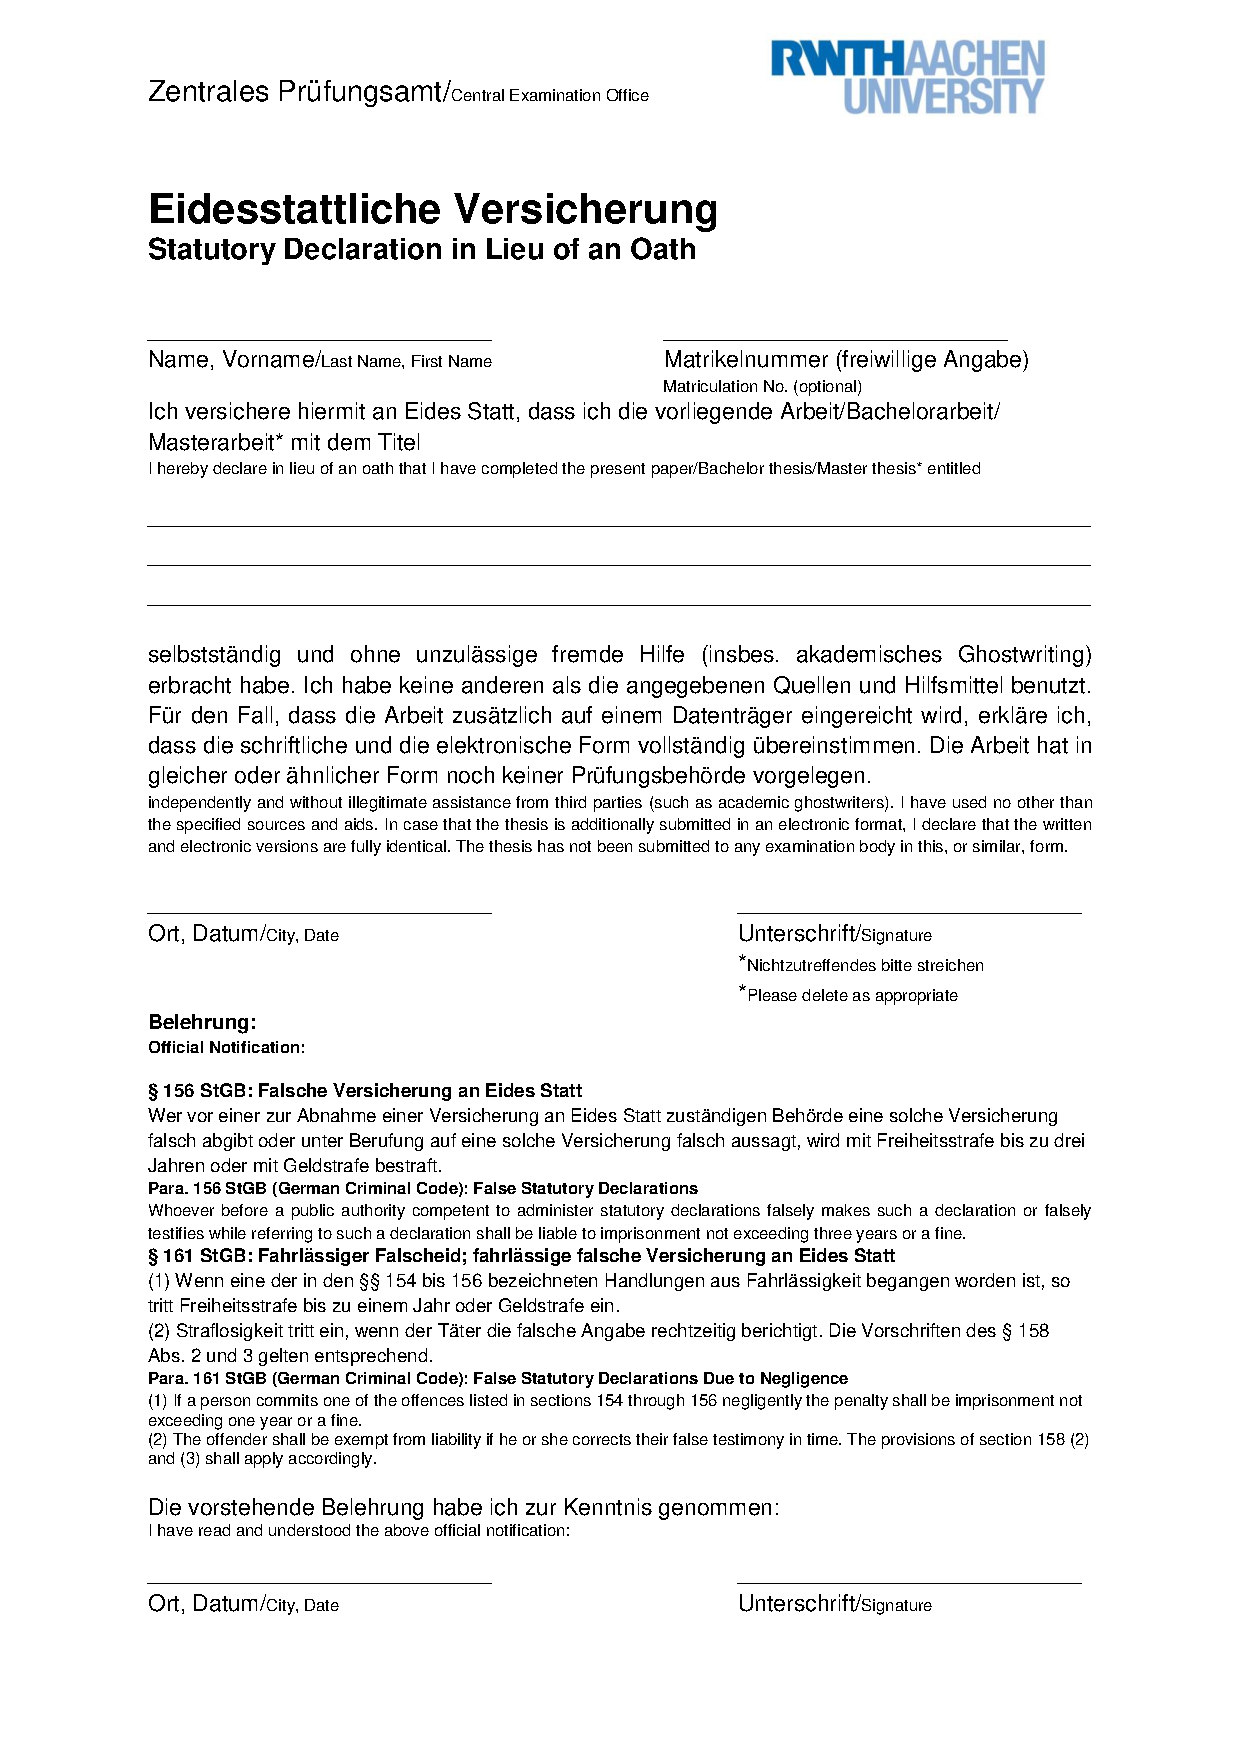
\includegraphics[width=\paperwidth]{oathstatement}}}
  \strut
\end{titlepage}

%% %%%%%%%%%%%%%%%%%%%%%%%%%%%%%%%%%%%%%%%
%% old version of declaration, not used anymore!!!
%
% ~
% \vfill
% I hereby declare that I have created this work completely on my own
% and used no other sources or tools than the ones listed,
% and that I have marked any citations accordingly.
%
% Hiermit versichere ich, dass ich die vorliegende Arbeit selbst\"andig
% verfasst und keine anderen als die angegebenen Quellen und Hilfsmittel
% benutzt sowie Zitate kenntlich gemacht habe. 
%
%\begin{flushright}
%\vspace{12mm}
%$\overline{Aachen, MONTH \mathit{YEAR}}$\\
%\textit{YOUR NAME}
%\end{flushright}
%% %%%%%%%%%%%%%%%%%%%%%%%%%%%%%%%%%%%%%%%
%\emptydoublepage

\setcounter{page}{5}

%% %%%%%%%%%%%%%%%%%%%%%%%%%%%%%%%%%%%%%%%%%%%%%%%%%%%%%%
%%  Table of Content
%% %%%%%%%%%%%%%%%%%%%%%%%%%%%%%%%%%%%%%%%%%%%%%%%%%%%%%%
\tableofcontents
\emptydoublepage

%% %%%%%%%%%%%%%%%%%%%%%%%%%%%%%%%%%%%%%%%%%%%%%%%%%%%%%%
%%  List of Figures
%% %%%%%%%%%%%%%%%%%%%%%%%%%%%%%%%%%%%%%%%%%%%%%%%%%%%%%%
\listoffigures
\emptydoublepage

%% %%%%%%%%%%%%%%%%%%%%%%%%%%%%%%%%%%%%%%%%%%%%%%%%%%%%%%
%%  List of Tables
%% %%%%%%%%%%%%%%%%%%%%%%%%%%%%%%%%%%%%%%%%%%%%%%%%%%%%%%
\listoftables
\emptydoublepage



%% %%%%%%%%%%%%%%%%%%%%%%%%%%%%%%%%%%%%%%%%%%%%%%%%%%%%%%
%%  Abstract
%% %%%%%%%%%%%%%%%%%%%%%%%%%%%%%%%%%%%%%%%%%%%%%%%%%%%%%%
%%  the abstract should breifly describe the work
%%
\thispagestyle{empty}
% %%%%%%%%%%%%%%%%%%%%%%%%%%%%%%%%%%%%%%%%%%%%%%%%%%%%%%%%%%%%%%%%%%%%%%%%%%%%
%  This file is part of the iTec thesis template used at the
%  Chair Individual and Technology at RWTH Aachen University.
% %%%%%%%%%%%%%%%%%%%%%%%%%%%%%%%%%%%%%%%%%%%%%%%%%%%%%%%%%%%%%%%%%%%%%%%%%%%%

%\loadgeometry{myAbstract}

%% %%%%%%%%%%%%%%%%%%%%%%%%%%%%%%%%%%%%%%%%%%%%%%%%%%%%%%%%%%%%%%%%%%%%%
%\chapter*{Abstract\markboth{Abstract}{Abstract}}
\chapter*{Abstract}
% we need to add the abstract to the toc manually
\addcontentsline{toc}{chapter}{\protect\numberline{}Abstract}
\label{chap:abstract}

Large Language Models (LLMs) are increasingly employed in political simulations, but most existing research has largely focused on two-party systems such as the United States. This paper extends the scope to a multi-party democracy, using Germany as a case study. We simulate dyadic debates between LLM agents assigned realistic political personas derived from the German Longitudinal Election Study (GLES), with initial positions benchmarked against official party stances from the Wahl-O-Mat. Using the SAUCE framework (Neuberger et al., 2024), we generate and analyse 2,800 debates to investigate (1) whether LLM agents with strong partisan affiliation align with their party’s official positions, and (2) whether discussions cause systematic opinion shifts and convergence. To ensure robustness, we apply three different prompt versions and compare their effects on agent opinions. Results show that prompt design significantly affects responses, underscoring the need for careful experimental control. Despite this sensitivity, our findings indicate that agents often begin aligned with party positions but exhibit opinion shifts over time, with evidence of convergence towards more uniform stances. These findings highlight both the potential and the limitations of using LLM agents as proxies for political opinion dynamics in multi-party contexts, offering methodological contributions for computational social science and raising questions about hidden biases in LLM-based simulations.
\emptydoublepage

%% %%%%%%%%%%%%%%%%%%%%%%%%%%%%%%%%%%%%%%%%%%%%%%%%%%%%%%
%%  Acknowledgements
%% %%%%%%%%%%%%%%%%%%%%%%%%%%%%%%%%%%%%%%%%%%%%%%%%%%%%%%
%%  time to say thank you to everybody you feel grateful
%%
\thispagestyle{empty}
\include{acknowledgements}
\emptydoublepage

%In der Arbeit verwendete Konventionen (Formelsatz, Definitionen, etc.)
%conventions applied in the thesis (AE/BE, definitions, etc.)
\include{conventions}
\emptydoublepage

%--------------------------------------------------------------
\mainmatter

% %%%%%%%%%%%%%%%%%%%%%%%%%%%%%%%%%%%%%%%%%%%%%%%%%%%%%%%%%%%%%%%%%%%%%%
%  ╭─────────╮                      ╔══╦╗ ╗ ╔═╦═╗ ╥ ┌─┐┌─┐┌─┐┬ ┬┌─┐┌┐ ┬
%  │ ,-= ━━━┑│                  |   ╠═╦╝╚╗╠╗║ ║ ╠═╣ ├─┤├─┤│  ├─┤├─ │└┐│
%  │ % iTec  │                  |   ╨ ╚═ ╚╝╚╝ ╨ ╨ ╨ ┴ ┴┴ ┴└─┘┴ ┴└─┘┴ └┘
%  │┃°. .°.  │ Chair Individual |          ┬ ┬┌┐ ┬┬┬  ┬┌─┐┬─┐┌─┐┬┌┬┐┬ ┬
%  │┖  °   ° │   and Technology |          │ ││└┐││└┐┌┘├─ ├┬┘└─┐│ │ └┬┘
%  ╰─────────╯                             └─┘┴ └┘┴ └┘ └─┘┴└─└─┘┴ ┴  ┴
% %%%%%%%%%%%%%%%%%%%%%%%%%%%%%%%%%%%%%%%%%%%%%%%%%%%%%%%%%%%%%%%%%%%%%%
%  This file is part of the Master's thesis LaTeX template used at the
%  Chair Individual and Technology (iTec) at RWTH Aachen University.
% %%%%%%%%%%%%%%%%%%%%%%%%%%%%%%%%%%%%%%%%%%%%%%%%%%%%%%%%%%%%%%%%%%%%%%

%% %%%%%%%%%%%%%%%%%%%%%%%%%%%%%%%%%%%%%%%%%%%%%%%%%%%%%%%%%%%%%%%%%%%%%
\chapter{Introduction}
\label{chap:introduction}

\section{Context and Motivation}

Large Language Models (LLMs) such as GPT  \citep{brown2020language} or Mistral \citep{jiang2023mistral7b} have rapidly evolved from simple text predictors into complex conversational agents capable of reasoning, debating, and simulating social interaction. Their ability to generate coherent, persuasive, and context-aware arguments has led to increasing interest in using LLMs to study communication dynamics, decision-making, and even human-like social behaviour. Within computational social science, these models offer a unique opportunity: they allow controlled, repeatable simulations of debates that are otherwise difficult to study empirically with humans.

However, this opportunity comes with risks. Despite their fluency, LLMs inherit and sometimes amplify social biases present in their training data. Research has already shown that such models can display systematic patterns of gender, racial, and ideological bias in text generation, evaluation, and interaction. When deployed in multi-agent settings, such as in simulate debates or discussions, these biases may subtly affect how arguments are presented, whose perspectives appear more dominant, or which positions seem more persuasive.

Understanding such effects is crucial not only for assessing the fairness of LLM-driven systems but also for improving their interpretability as tools in social simulation. If an LLM debate environment systematically treats gendered personas differently, it may distort results, reinforcing stereotypes rather than modelling neutral discourse. Investigating these dynamics therefore matters both for advancing methodological rigour in computational social systems and for ensuring that the use of LLMs in social contexts remains transparent, responsible, and scientifically grounded.


\section{Problem Statement and Research Gap}

Recent advances in large language models (LLMs) have made it possible to simulate complex social phenomena such as political debates through multi-agent interactions. These simulations promise a controlled and reproducible way of studying opinion formation and persuasion processes—key interests in computational social science. However, while LLMs can generate coherent dialogue, the extent to which their simulated behaviours reliably reflect the intended social constructs rather than artefacts of the underlying models remains unclear.

A recent contribution in this area is the work by \citet{taubenfeld_systematic_2024}, who investigated systematic biases in simulated dyadic and triadic debates between LLM-based agents. Their framework paired agents with opposing ideological profiles (Republican, Democrat, and Default) and analysed how their expressed opinions evolved over multiple dialogue turns when debating controversial topics (\textit{Gun Violence, Racism, Climate Change, and Illegal Immigration}). The study found that, despite being instructed to represent distinct viewpoints, agents tended to converge in their opinions. When instructed to represent the same viewpoint, however, their opinions gradually shifted. The authors hypothesised that this behaviour reflects the underlying bias of the base model and noted that this goes against the common theory of echo chambers, where agents with like-minded views would tend to intensify their beliefs when interacting with each other.

To test this hypothesis, the authors fine-tuned separate versions of the model to adopt either a Democratic or Republican perspective. This process involved (1) generating 20 Democratic and 20 Republican personas, (2) prompting these personas to answer 100 politically themed questions designed to elicit their beliefs and reasoning, and (3) fine-tuning the base model on the resulting 2,000 responses using a parameter-efficient QLoRA next-word prediction task.

With these Democratic- and Republican-tuned models, the authors repeated the debate simulations. The results showed not only continued convergence between agents but, crucially, convergence towards the ideological direction of the fine-tuned model. This outcome strengthened the hypothesis that LLM debate behaviour is shaped more by the base model’s internal bias than by the explicit persona instructions given to the agents.

While the study established an important foundation, several broader questions remain open. First, the degree to which LLM behaviour depends on prompt design is largely unexplored. Subtle differences in phrasing, politeness, or structural cues could influence how agents interpret their roles and respond to debate topics, yet most studies—including that of \citet{taubenfeld_systematic_2024}—use a single prompt structure without assessing its robustness.

Second, the dynamics of opinion change observed in debate settings require a more quantitative treatment. The original analysis relied primarily on qualitative interpretation of plotted opinion trajectories. It remains unclear whether the apparent convergence toward a shared stance represents meaningful interaction effects or merely reflects model-level bias.

Finally, the debate simulations examined by \citet{taubenfeld_systematic_2024} were restricted to a bipartisan context (Republican versus Democrat). Real-world political discourse, however, is often more complex, involving multiple parties and overlapping ideological positions. Extending such analyses to a multi-party system would provide a more comprehensive test of LLMs’ ability to sustain diverse and stable viewpoints.

In addition, the original study relied on now outdated models (\texttt{gpt-3.5-turbo-instruct}, \texttt{Mistral 7B}, and \texttt{Solar 10.7B}), raising questions about whether the observed effects persist in more recent architectures. Addressing these methodological and conceptual gaps is crucial for understanding when and how LLM-based debate simulations can serve as valid tools for social-scientific inquiry.


\section{Research Questions}
\label{sec:research_questions}
While prior work often relies on a single debate prompt, subtle linguistic variations can alter how an LLM interprets its role and responds to contentious topics. This question examines whether different prompt phrasings—while keeping the underlying task identical—lead to measurable differences in agents’ expressed opinions. Assessing prompt sensitivity is essential for determining the robustness and reproducibility of LLM-based debate simulations. This leads to the first research question:
\researchquestion{RQ1: Is there a significant impact of the prompt chosen on the opinions?}



Unlike previous studies that constructed political personas through ad-hoc prompting, this study derives personas empirically from the German Longitudinal Election Study (GLES) dataset. These data-driven personas allow for a more grounded representation of real-world political attitudes. This second reseach-question therefore tests whether LLM agents initialised with empirically informed political profiles maintain ideological consistency with their affiliated party when engaged in debate and is formulated as follows.
\researchquestion{RQ2: Do agents with strong party affiliation align with their party’s official stance?}  


Earlier findings by \citet{taubenfeld_systematic_2024} indicated that LLM agents tend to converge in opinion, even when representing opposing sides. This question revisits that phenomenon using newer models and an extended multi-party debate framework. The aim is to quantify whether opinion change over time reflects genuine conversational influence between agents or merely the manifestation of shared underlying model bias.
\researchquestion{RQ3: Does discussion cause agents' opinions to significantly shift from their starting points and converge towards more uniform stances?}  




\section{Approach Summary}

This study simulates dyadic political debates between Large Language Model (LLM) agents endowed with socio-demographic and political profiles derived from the German Longitudinal Election Study (GLES). The methodological pipeline consists of six main stages (Figure~\ref{fig:approach_overview}):

\begin{figure}[h]
\centering
\begin{tikzpicture}[
    node distance = 14mm and 10mm,
    every node/.style = {align=center, font=\small, rounded corners, minimum height=1.1cm, text width=3.2cm, draw=black!70, fill=gray!5},
    arrow/.style = {->, thick, >=latex, black!70}
]

% Top row
\node (step1) {1. Agent Profiling \\ and Sampling};
\node (step2) [below=of step1] {2. Topic \\ Selection};
\node (step3) [right=of step2] {3. Debate \\ Pairing Design};

% Bottom row
\node (step5) [right=of step3] {5. Debate Simulation \\ and Data Collection};
\node (step4) [above=of step5] {4. Prompt Construction \\ and Sensitivity};
\node (step6) [below=of step5] {6. Validation \\ and Statistical Analysis};

% Arrows (top row)
\draw[arrow] (step1) -- (step3);
\draw[arrow] (step2) -- (step3);

% Arrows (bottom row)
\draw[arrow] (step4) -- (step5);
\draw[arrow] (step5) -- (step6);

% Vertical connectors
\draw[arrow] (step3) -- (step4);

\end{tikzpicture}
\caption{Overview of the six-stage methodological pipeline. }
\label{fig:approach_overview}
\end{figure}


\begin{enumerate}
    \item \textbf{Agent Profiling and Sampling:}  
    Personas are generated using the principle of \emph{Quantitative Persona Creation} \citep{Salminen2020quantative}. Each persona represents an archetypical supporter of one of six German political parties (CDU/CSU, SPD, Bündnis 90/Die Grünen, FDP, AfD, Die Linke), based on socio-demographic and attitudinal variables from the GLES 2021 dataset. A default, non-biographical agent serves as a baseline reference.

    \item \textbf{Topic Selection:}  
    Debate topics are drawn from five politically salient statements taken from the 2021 \emph{Wahl-O-Mat}, Germany’s official voter-assistance tool. These topics were selected to cover a range of policy domains and to elicit divergent party opinions.

    \item \textbf{Debate Pairing Design:}  
    Agents are paired across all within- and between-party combinations, including debates with the default agent. Each pair discusses all five topics, leading to a comprehensive coverage of ideological interactions.

    \item \textbf{Prompt Construction and Sensitivity Conditions:}  
    To examine the robustness of model responses, three prompt formulations—varying in conciseness, descriptiveness, and politeness—are applied to two use cases: debate continuation and questionnaire evaluation. This results in six total prompt skeletons (see Table~\ref{tab:prompt_skeletons}).

    \item \textbf{Debate Simulation and Data Collection:}  
    Debates proceed for 20 alternating turns using a modified version of the SAUCE framework \citep{neuberger2024sauce}. Every fourth turn, both agents are queried with a Likert-style evaluation of the current topic to capture temporal opinion shifts. Across all conditions, this yields 21,000 individual measurements.

    \item \textbf{Validation and Statistical Analysis:}  
    To assess the validity of the generated Likert responses, a subset of outputs is evaluated by human annotators. The main quantitative analyses employ mixed-effects models to test for effects of prompt version, debate partner, and time on agents’ expressed opinions, accounting for repeated measures within debate sessions.
\end{enumerate}

This multi-stage design ensures a systematic investigation of (i) ideological alignment, (ii) opinion shift dynamics, and (iii) prompt sensitivity across different LLM architectures and interaction contexts.



\section{Main Contributions}

This thesis contributes to the emerging field of LLM-based social simulations by extending existing debate frameworks both conceptually and methodologically. Building on \citet{taubenfeld_systematic_2024}, it introduces several innovations that enhance the validity, robustness, and generalizability of such simulations.

First, the study systematically investigates prompt robustness. While prior work typically relied on a single debate prompt, this thesis varies the linguistic framing of prompts while keeping all other parameters constant. This enables an empirical assessment of how sensitive debate outcomes are to subtle differences in wording, and whether observed opinion differences stem from genuine model bias or the phrasing of the task itself.

Second, it develops an empirical method for persona construction. Instead of generating political profiles through ad-hoc instructions, the personas used in this study are derived from the German Longitudinal Election Study (GLES) dataset. This approach grounds the agents’ ideological orientations in real-world survey data, creating a reproducible and data-driven foundation for representing political attitudes.

Third, the thesis extends the traditional bipartisan debate setup to a multi-party framework that mirrors the diversity of the German political landscape. This expansion allows for a more realistic and fine-grained analysis of ideological alignment, cross-party convergence, and the stability of multiple competing viewpoints within the same discussion.

Finally, the study introduces a quantitative approach to opinion dynamics using mixed-effects models. This enables a statistical assessment of whether debates lead to significant opinion shifts and whether convergence arises from conversational influence or shared underlying model bias. In doing so, the analysis moves beyond qualitative interpretation towards a more rigorous, data-driven understanding of interaction effects.

Together, these contributions advance the methodological toolkit for studying social phenomena through language model interactions and help clarify under what conditions LLM debates can serve as valid approximations of human political discourse.



\section{Thesis outline}


%\emptydoublepage

% %%%%%%%%%%%%%%%%%%%%%%%%%%%%%%%%%%%%%%%%%%%%%%%%%%%%%%%%%%%%%%%%%%%%%%
%  ╭─────────╮                      ╔══╦╗ ╗ ╔═╦═╗ ╥ ┌─┐┌─┐┌─┐┬ ┬┌─┐┌┐ ┬
%  │ ,-= ━━━┑│                  |   ╠═╦╝╚╗╠╗║ ║ ╠═╣ ├─┤├─┤│  ├─┤├─ │└┐│
%  │ % iTec  │                  |   ╨ ╚═ ╚╝╚╝ ╨ ╨ ╨ ┴ ┴┴ ┴└─┘┴ ┴└─┘┴ └┘
%  │┃°. .°.  │ Chair Individual |          ┬ ┬┌┐ ┬┬┬  ┬┌─┐┬─┐┌─┐┬┌┬┐┬ ┬
%  │┖  °   ° │   and Technology |          │ ││└┐││└┐┌┘├─ ├┬┘└─┐│ │ └┬┘
%  ╰─────────╯                             └─┘┴ └┘┴ └┘ └─┘┴└─└─┘┴ ┴  ┴
% %%%%%%%%%%%%%%%%%%%%%%%%%%%%%%%%%%%%%%%%%%%%%%%%%%%%%%%%%%%%%%%%%%%%%%
%  This file is part of the Master's thesis LaTeX template used at the
%  Chair Individual and Technology (iTec) at RWTH Aachen University.
% %%%%%%%%%%%%%%%%%%%%%%%%%%%%%%%%%%%%%%%%%%%%%%%%%%%%%%%%%%%%%%%%%%%%%%


%% %%%%%%%%%%%%%%%%%%%%%%%%%%%%%%%%%%%%%%%%%%%%%%%%%%%%%%%%%%%%%%%%%%%%%
\chapter{(Theoretical) Background and Related Work}
\label{chap:background_related-work}


\section{Large Language Models}
\label{sec:llm}
\subsection{Model architecture}
Large Language Models (LLMs) are machine leaning models based on the Transformer Architecture which was first introduced by \citet{vaswani2017attention} and came proceeding developments in sequence modelling such as LSTMs \citep{hochreiter1997long} and (gated) Recurrent Neural Networks (RNN) \citep{cho2014learning}. Transformer models rely completely on self-attention to compute representations of its input and output without using sequence-aligned RNNs or convolutions. These leads to major gains with regards to the parallelisation of computation and long-range dependencies of the input text \cite{kimDHR17}. 

In this process of exploring RNNs for machine translation and text summarisation the concept encoder-decoder structure was developed \cite{sutskever2014sequence}. The encoders will take the input being a embedding sequence $X$ which consists of the input and the positional encoding and creates an intermediate vector $Z$ which can then be processed by the decoder. Additionally the decoder will also get the previously self-generated output token as an input.


Building on the transformer architecture \citep{radford2018improving} created a new approach using the unsupervised pre-training + supervised fine-tuning paradigm. This is done by applying a generative pre-training on a the transformer, which is then followed by a discriminative fine-tuning on a specific task. The advantage of this was that due to the model already having the casual relationships inside one was able to fine-tune the model with a lot smaller datasets. Combining unsupervised with supervised techniques is in itself not novel and has already previously been used for sequence labelling or text classification \cite{van2020survey, yarowsky1995unsupervised}.


Unlike encoder-decoder models, which process the entire input before generating output, GPT models rely only on a decoder with causal masking. This allows them to generate text sequentially while maintaining coherence over long contexts \ref{fig:decoder} \cite{radford2018improving,brown2020language}. The decoder will given sequence of tokens $(x_{i-k},...,x_{i-1})$ predict or classify token $x_i$. 


\begin{figure}
    \centering
    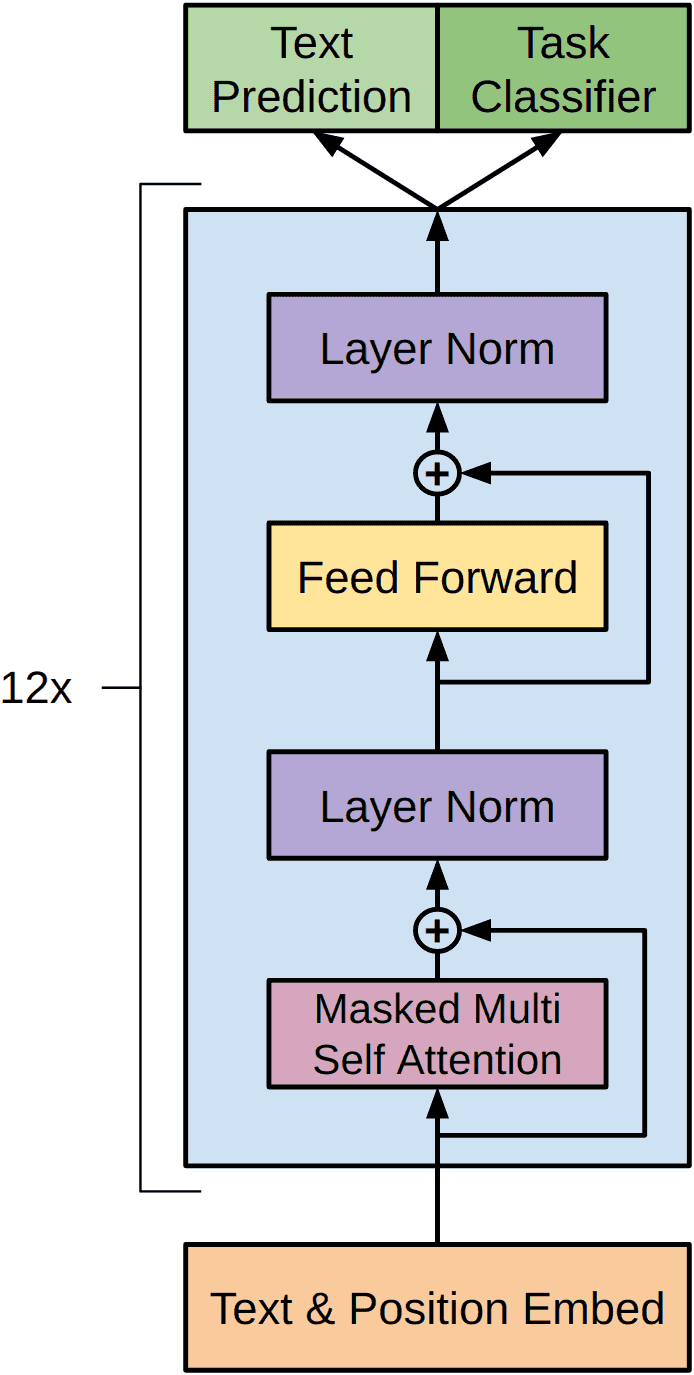
\includegraphics[width=0.5\linewidth]{imgs/decoder.png}
    \caption{Decoder structure proposed by \citet{radford2018improving}}
    \label{fig:decoder}
\end{figure}



The attention mechanism contains 
The mentioned attention is symbolised by the formula \ref{for:attention}, where Q is the query, K is the Key and V is is value. 
\begin{align}
\label{for:attention}
    \text{Attention}(Q,K,V) &= softmax(\frac{QK^T}{\sqrt{d_k}})V
\end{align}


Rather then just having a single attention \cite{vaswani2017attention} create a concept called multi-headed-attention which can be seen in formula \ref{for:multiHead}. Having a multi-headed-attention allows for different attention heads to focus on different aspects of the input. This type of model also allows for highly parallelised training and inference of the data \citep{min2023recent}. 

\begin{align}
\label{for:multiHead}
    \text{MultiHead}(Q,K,V) &= Concat(head_1, head_2 ... , head_h)W^0 \\
    \text{where head}_i &= \text{Attention}(QW_i^Q,KW^K_i, VW^V_i)
\end{align}



\subsection{Alignment fine tuning RLTH}
\label{sub:alignment}

When using LLMs for generating text they will in their pre fine-tuned state find the token which has the highest likelihood of appearing. This behaviour might be different from the users expected behaviour which would often be that the LLM "follow the user’s instructions helpfully and safely" \cite{ouyang2022training}. This could result in "misaligned" behaviour such as making up facts, generating biased or toxic text, or simply not following user instructions \cite{bommasani2021opportunities, bender2021dangers, kenton2021alignment} \todo{add the citation to the specific part of the sentence (find source in "Training language models to follow..."}, a term coined by \citet{ouyang2022training}.

To combat this misalignment they applied a system called reinforcement learning from human feedback (RLHF \cite{christiano2017deep}). This technique follows a three step procedure, firstly prompt taken from the API interface were taken and humanly annotated. This annotation was then used to train the model. Secondly, this model was then used to generate output based on another batch of prompts. In this step the human annotator would rank the output. This output was then used to generate a reward model. This is a much smaller (6B parameter in comparison to the 175B of GPT-3). Finally the LLM will be prompted again and the reward model will calculate the reward for this output. The reward is then used to update the policy using proximal policy optimization \cite{ouyang2022training}.

This technique used for fine-tuning resulted in many different positive results, such as that labellers significantly preferred the with RLHF fine-tuned model over the non-fined-tuned version even if the non-fined-tuned version was a lot larger, 

The model the researches applied RLHF on, InstructGPT, significantly outperforms the base model, GPT-3, in following instructions, with labellers preferring its responses. The 1.3B InstructGPT is rated higher than the 175B GPT-3, and the 175B InstructGPT is preferred 85\% of the time over GPT-3. It generates more appropriate, truthful, and constraint-following responses, reducing hallucination rates by about half. While InstructGPT slightly reduces toxicity, no effect was found with regards to social and gender biases\cite{ouyang2022training}.






\section{Bias in LLMs}
\label{sec:gender-bias-in-llm}

\subsection{Definition}

But what is social bias? Social Biases are very broad and can be observed in multiple different facets. In the taxonomy by \citet{gallegos_bias_2024} (table \ref{tab:harms}) social biases are subdivide it into two different groups. The first group representational harms contain misrepresentation, stereotyping, disparate system performance, derogatory language, and exclusionary norms and the second group allocational harms contain direct discrimination and indirect discrimination. It is important to notice that these groups are not exclusive and that the exclusionary norms may turn into allocational harms. For example by associating “Muslim” with “terrorist” could lead to an LLM-aided resume screening to hold preferences for non-Muslims. \todo{maybe change to woman maths example}



\subsection{Sources of bias}

Bias is deeply embedded in the real world, shaping institutions, social structures, and digital spaces. Institutional biases often stem from historical and systemic inequalities, where certain social groups face disadvantages. The internet, despite its open accessibility, is not an accurate reflection of society. For example, Wikipedia's contributor demographics illustrate this disparity: while women make up 49\% of Wikipedia readers in the U.S., only an estimated 22.7\% of adult contributors are female \cite{hill2013wikipedia}. Such imbalances can be found in many other websites and are made more sevear by phenomena like homophily (the tendency of individuals to interact with similar others \cite{karimi2018homophily}) and algorithmic feedback loops(reinforce biases through mechanisms like search engine ranking \cite{lerman2014leveraging}). Additionally, demographic factors such as age, education, and socioeconomic status further influence online engagement, shaping the data that algorithms rely upon.

LLMS inherit these biases from the data they are trained on. Modern AI systems require vast amounts of data, and their capabilities are directly tied to the information they are fed on. In the case of LLMs, training data is predominantly sourced from the internet, often through large-scale web crawls like Common Crawl \cite{brown2020language}. However, the web itself is skewed—only a fraction of individuals actively contribute content, meaning that the perspectives represented online are neither neutral nor fully inclusive. For instance, product reviews, forum discussions, and social media posts are authored by a self-selected subset of users, leading to an overrepresentation of certain opinions while others remain underrepresented.

\subsection{Detection}


A wide variety of methods has been created to detect and measure the bias in LLMs. These generally fit into three categories, embedding based, portability based and Generated Text based \cite{gallegos_bias_2024}.


\subsubsection{Embedding Based Metrics (EBM)}
Here one looks at the vector embeddings of the words or of sentences. For example one could compare the cosine distance from the vector of the tokens for \texttt{doctor, nurse, man} and \texttt{woman}. With the assumption that unbiased embeddings should have similar cosine similarity to opposing social group terms  (Word Embedding Association Test \cite{caliskan2017semantics}). Modification from this, where one either takes the normalised sum of the vectors (Sentence Bias Score \cite{dolci2023improving}) or one takes the vector of the sentence (Sentence Encoder Association Test\cite{may2019measuring}) also exist. This technique comes with serious shortcomings since the the correlation between the found bias found in the embedding space and the bias found in the downstream application is very weak to non existent \cite{goldfarb2021intrinsic,cao2021holistic}. 

\subsubsection{Probability Based Metrics (PBM)}
Probability-based metrics assess bias by analysing how likely a model is to generate certain tokens or sentences. One approach would mask a part of the word and see which the likelihoods of words which would be chosen by the model \cite{webster2020measuring}. More sophisticated versions with normalisation also exist (Log-Probability Bias Score \cite{kurita2019measuring}).

Another group of methods, the Pseudo-Log-Likelihood Methods, such as the Context Association Test or CrowS-Pairs Score compare the likelihood of two sentences with a word changed. An example would be comparing the likelihood between "One wouldn't expect this discovery from a \textbf{Female} astrophysicist" and "One wouldn't expect this discovery from a \textbf{Male} astrophysicist". 

Again her only weak correlation can be found though between the PBM and the downstream task \cite{kaneko2022debiasing, delobelle2022measuring}. \citet{goldfarb2023prompt} observed that 68\% of the papers applying bias tests used EBMs or PBMs (only observing upstream tasks).

\subsubsection{Generated Text-Based Metrics}
\label{subsubsec:generated-text-based-metrics}

The final category assess bias by analysing the outputs a model produces when prompted with different inputs. Thus treating the model as a black box.


\citet{gallegos_bias_2024} subdivided this into three different under-categories, distribution of output words, classifier and lexical based metrics. The Distribution-based metrics are used to analyse the distribution of tokens generated, by the LLM depending on the social group. The standard approach for this is that the LLM is prompted to, given a set of input tokens, a continuation of these. For example the Co-Occurrence score calculates the likelihood of words appearing more frequently in either female or male contexts \cite{bordia2019identifying}. There are a number of similar measurements which all work fairly similar such as the Demographic Representation \cite{liang2022holistic}, Stereotypical Associations \cite{liang2022holistic}, and Marked Persons \cite{cheng2023marked}.

The classifier sub-category of metrics use a second model to evaluate the output of the LLMs. Using a toxicity classifier one can evaluate either the mean toxicity score \cite{gehman2020realtoxicityprompts}, the ratio of outputs with a toxicity over a threshold \cite{liang2022holistic}. A similar approach can be used with regards to sentiment \cite{huang2019reducing,sheng2019woman}. The second model may also be trained on specific tasks, by generating a dataset based on different dimensions of sexism \citet{samory2021call} trained a logid, CNN, and fine-tuned a BERT language model. These resulting models all outperformed the baseline which was given by the Jigsaw’s Perspective API \cite{PerspectiveAPI2024} which is widely used  \cite{gehman2020realtoxicityprompts,liang2022holistic}

Third, lexical metrics provide a way to assess bias by analysing the language used in a model's generated output. Words can be mapped to predefined values, such as hurtfulness scores \cite{nozza2021honest}, psycholinguistic norms \cite{dhamala2021bold}, which include attributes like dominance, sadness, or fear, or the presence of gendered language \cite{dhamala2021bold}.

Each of these metrics come with associated shortcomings. With the distribution based metrics the co-occurrences between the input and protected attitude might be a poor proxy for downstream disparities. For example, co-occurrence can occur through a lot of counterspeach \cite{gligoric2024nlp}. The classifier categories will always only be as reliable as the model which is analysing the output. If there are biases in the auxiliary model the evaluation of the output might also have that bias. And with the final group, lexicon-based metrics, the issue exists that the lexicon can not understand words in the context.




\section{Multi-Agent Systems} 

Multi-agent systems (MAS) study interactions between autonomous agents that cooperate, compete, or coexist within a shared environment. A common definition describes MAS as "systems that include multiple autonomous entities with either diverging information or diverging interests, or both" \cite[p.xiii]{shoham2008multiagent}. These systems are widely applied in robotics, economics, artificial intelligence, and distributed computing \cite{wooldridge2009introduction}. Unlike single-agent models, MAS focus on coordination, negotiation, and decentralized decision-making, often drawing from game theory, logic, and reinforcement learning \cite{stone2010ad}.

Whereas early research on MAS explored rule-based and logic-driven frameworks \cite{shoham2008multiagent}, modern approaches increasingly focus machine learning and large language models for adaptive agent behaviour \cite{baker2019emergent}. The combination of LLms and MAS has been widely explored recently with simulations ranging such as economical theories \cite{zhao2023competeai} or simulating real time social interaction \cite{kaiya2023lyfe}. 

When replicating psychological experiments with human participants LLM  have showed similar results \cite{cui2024can, aher2023using} to these. It is very important in this case to mention that LLMs are also trained on the experiments tested of these papers which make the results unsurprising. Some social phenomena are also not reproducible by using LLM agents. 

\subsection{Dyadic Debates}

In the experiment by \citet{taubenfeld_systematic_2024} they set up dyadic and triadic discussion between LLM agents. The agents were subdivided into three categories, democrats, republicans, and control. When debating on topics which majority of the supporters of the parties don't agree upon (\textit{Gun Violence, Racism, Climate Change, and Illegal Immigration}) it was observed that the opinion of the LLMs agents approaches the inherent bias of the LLM over the course of the debate. This shift could also be observed when two supporters of the same political party had a similar stance to one of the topics. That the opinions shift towards the bias of the model was validated by changing the bias of the model by finetuning it to be behave more republican or democrat. To measure the opinion shift in the LLM the agents were asked to state how much they agree on a statement and give their answer from a value between 0 and 10. The framework the authors used to model the agents was the SAUCE framework \cite{neuberger2024sauce}.


This behaviour of converging towards to less polarisation contradicts the echo chamber theory. The echo chamber theory states that when individuals with shared opinions come together there views will intensify. Using digital trace data this has behaviour has been shown in numerous settings in Social Networks \cite{terren2021echo}. \citet{terren2021echo} also looked at papers which used self-reporting as a method to observe the phenomena and found very mixed to no evidence of echo-chambers in social networks. The effect of echo chamber are also to be found in offline settings. \citet{hobolt2024polarizing} formed groups of nationally representative partisans and assign them to discuss a salient policy issue, either with like-minded partisans (an echo chamber) or in a mixed-partisan group. The homogenous groups had an increase of polarisation than the mixed groups.

\subsection{Left-Leaning Bias}

Recent studies have explored the political biases present in large language models. \citet{rutinowski2024self} found that LLMs tend to exhibit a left-leaning bias when within Chat-GPT when asked to answer the questions posed by the political compass test. Similar results can be seen when prompting LLMs the question of the "Wahl-O-Mart", a voting advice application used in Germany \cite{rettenberger2025assessing}. The authors prompted the LLMs to answer the questionnaire which resulted in the finding that Larger Models , tend to align more closely with left leaning political parties, while smaller models often remain neutral, particularly when prompted in English. \todo{maybe more evidence?}

\subsection{Offline Dyadic Debates}

Dyadic Debates have also been analysed in offline settings with the focus of gender roles. \citet{bowles2010gender} set up dyadic debates in which participants had to negotiate over the price of an house, sometimes being in the role of the seller and sometimes in the role of the buyer. The negotiation always had participant and one confederate who where tasked to be very uncooperative with regards of finding a fair price. The persistence was measured using self-evaluation and the effect of the participants gender by the confederates gender on persistence was evaluated. Contrary to the stereotype, that men are less willing to compromise \cite{kray2001battle}, no significant result was found with between the reported gender and reported persistence. The confederates gender moderated though so that woman significantly persisted higher with male confederates. 




\section{Prompt Sensitivity}

Large Language Models (LLMs) are known to be highly sensitive to prompt design \cite{sclar2023quantifying, gao2020making, jiang2020can}. \citep{sclar2023quantifying} demonstrated that even minor, semantically irrelevant changes to prompt formatting can result in substantial variations in model accuracy, which was shown at an an strong example using LLaMA-2-13B. 

In response to such findings, several frameworks have been developed to systematically assess prompt sensitivity, including POSIX (PrOmpt Sensitivity IndeX) \citep{chatterjee2024posix} and ProSA \citep{zhuo2024prosa} which evaluate the variance of the output given differently formatted and framed input. Interestingly, using the ProSA framework, the authors found that larger model size does not necessarily imply greater robustness to prompt variations. For instance, LLaMA3-8B-Instruct outperformed the significantly larger Qwen1.5-72B-Chat on their sensitivity metric.

Consistent with the findings of \cite{chatterjee2024posix}, few-shot learning was shown to substantially reduce prompt sensitivity, suggesting that including even minimal context examples in the prompt can improve stability and output consistency.
%\emptydoublepage

% %%%%%%%%%%%%%%%%%%%%%%%%%%%%%%%%%%%%%%%%%%%%%%%%%%%%%%%%%%%%%%%%%%%%%%
%  ╭─────────╮                      ╔══╦╗ ╗ ╔═╦═╗ ╥ ┌─┐┌─┐┌─┐┬ ┬┌─┐┌┐ ┬
%  │ ,-= ━━━┑│                  |   ╠═╦╝╚╗╠╗║ ║ ╠═╣ ├─┤├─┤│  ├─┤├─ │└┐│
%  │ % iTec  │                  |   ╨ ╚═ ╚╝╚╝ ╨ ╨ ╨ ┴ ┴┴ ┴└─┘┴ ┴└─┘┴ └┘
%  │┃°. .°.  │ Chair Individual |          ┬ ┬┌┐ ┬┬┬  ┬┌─┐┬─┐┌─┐┬┌┬┐┬ ┬
%  │┖  °   ° │   and Technology |          │ ││└┐││└┐┌┘├─ ├┬┘└─┐│ │ └┬┘
%  ╰─────────╯                             └─┘┴ └┘┴ └┘ └─┘┴└─└─┘┴ ┴  ┴
% %%%%%%%%%%%%%%%%%%%%%%%%%%%%%%%%%%%%%%%%%%%%%%%%%%%%%%%%%%%%%%%%%%%%%%
%  This file is part of the Master's thesis LaTeX template used at the
%  Chair Individual and Technology (iTec) at RWTH Aachen University.
% %%%%%%%%%%%%%%%%%%%%%%%%%%%%%%%%%%%%%%%%%%%%%%%%%%%%%%%%%%%%%%%%%%%%%%


%% %%%%%%%%%%%%%%%%%%%%%%%%%%%%%%%%%%%%%%%%%%%%%%%%%%%%%%%%%%%%%%%%%%%%%
\chapter{Methods}
\label{chap:methods} 


\section{Overview}
We simulate dyadic political debates between Large Language Model (LLM) agents endowed with socio-demographic and political profiles derived from the German Longitudinal Election Study (GLES) and evaluate (i) initial alignment with official party stances, (ii) opinion shifts during interaction, and (iii) convergence dynamics. A preliminary prompt sensitivity experiment quantifies whether minor prompt formatting changes materially affect quantitative survey-style outputs (7-point Likert judgements of policy statements). All analyses use mixed-effects modelling to account for repeated measurements within debate sessions.

\section{Agent Profiling and Sampling}
\label{sec:agent_profiling_and_sampling}

The personas were generated based on quantitative measurements, which is referred to as Quantitative Persona Creation \cite{Salminen2020quantative}. Taking the approach from \cite{von2024vox}, we use data from the cumulative German Longitudinal Election Study (GLES) Cross-Section 2009–2017 \citep{ZA6835}. This dataset contains socio-demographic and political attitude data from German federal election years 2009, 2013, 2017, and 2021. This dataset  is then filtered by only taking respondents data which contain data for the variables of interest (see below). Furthermore, we only take the subset of the data which have the encoded field start set to \texttt{27.09.2021}, meaning that this survey was taken after the 2021 federal election and thus respondents can state which party they have voted for. This leads to a total of 3,431 respondents. The GLES records are filtered to retain agents with strong party identification (German: \emph{sehr stark}) for six Bundestag parties: CDU/CSU, SPD, Bündnis 90/Die Grünen, FDP, AfD, Die Linke which were the parties having seats in the 20th Bundestag between 2021 and 2025. The Party SSW is not included due to it only contesting in Schleswig-Holstein and only having a sigle seat in the Bundestag. 

The selected variables from which the personas were generated were taken from \cite{von2024vox} and have been shown to be important predictors of voting behaviour—demographics, party affiliations, and views on politically salient issues, such as immigration. The variables include age, gender, education, employment, household income, whether they live in west or east Germany, religiousness, self-evaluation of weather they see themselves as left or right leaning, party alignment, opinion on inequality, option on immigration and their 2021 federal election vote. The variables were then made into a story by using a template which can be seen in the Appendix \todo{add template into appendix}.

Furthermore we create a default agent which doesn't have a biography. This serves as a baseline  \todo{as a baseline for what????}

\section{Wahl-O-Mat Statements}

To chose the debate topics a subset of questions from the Wahl-O-Mat from the 2021 federal election was chosen. The Wahl-O-Mat is a digital tool designed to support voters in Germany in assessing how political parties align with their views. It’s typically released concerning a specific election. The user is presented with a series of political statements, ranging from social issues to economic policies, and covers a wide range of topics relevant to the political landscape at the time.


\begin{figure}
    \centering
    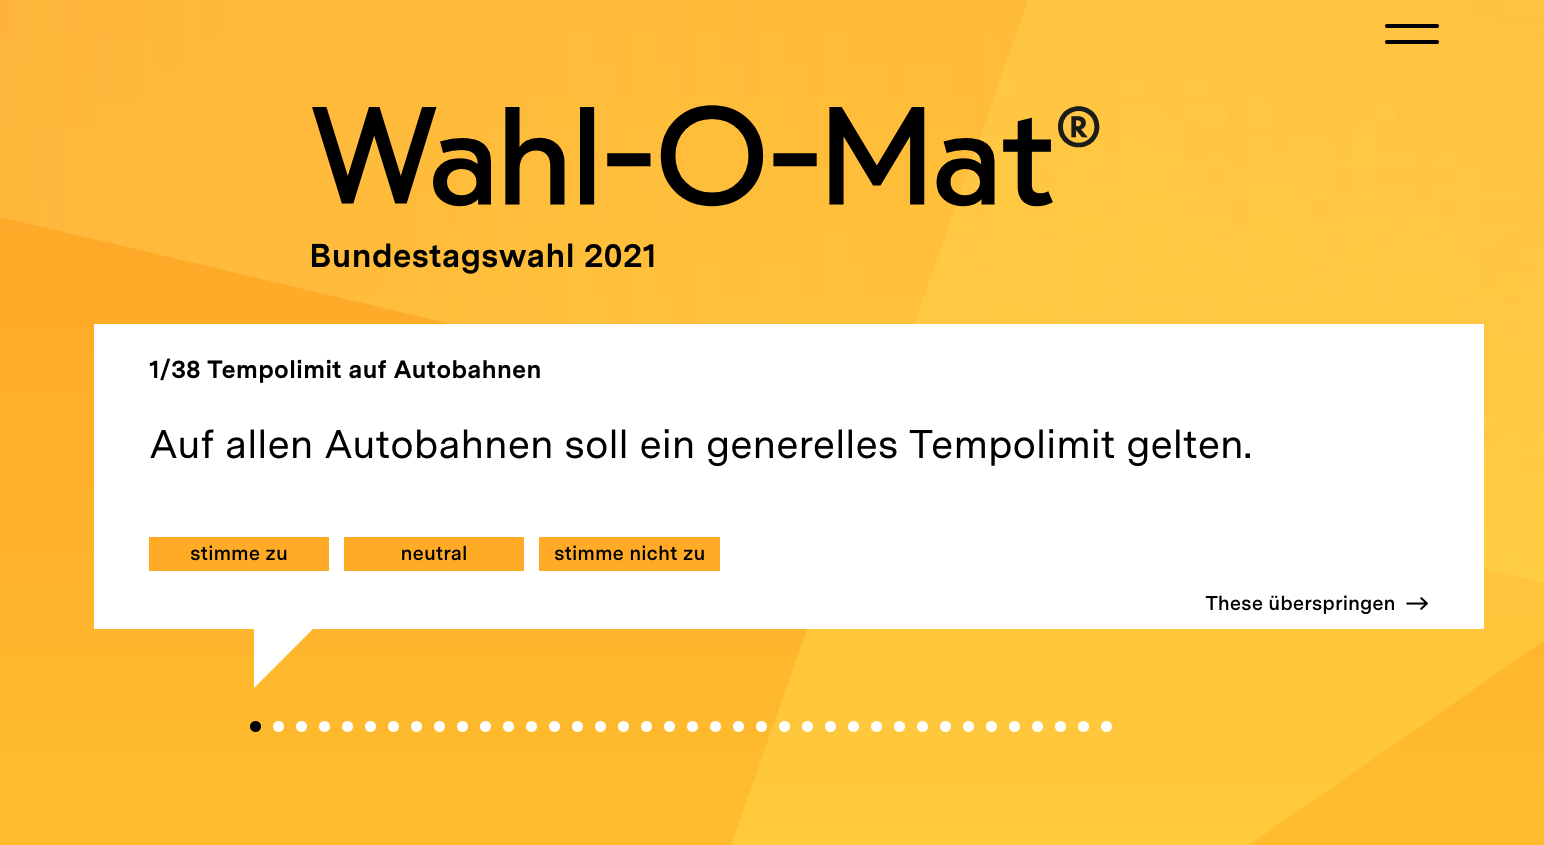
\includegraphics[width=0.9\linewidth]{imgs/Wahl-O-Mat-Tempo.png}
    \caption{A question of the 2021 Federal Election Wahl-O-Mat which translates to "A general speed limit should apply on al motorways"}
    \label{fig:Wahl-O-Mat}
\end{figure}



For each statement, the user can decide whether they agree, are neutral, or disagree (see Figure \ref{fig:Wahl-O-Mat}). In the end, the Wahl-O-Mat compares the user’s responses with the official positions of the political parties participating in the election. The Wahl-O-Mat then ranks the parties, showing which parties’ policies align most closely with the user’s positions. The Wahl-O-Mat was developed by the Federal Agency for Civic Education (FACE) and is considered the most important tool for electoral decision-making in Germany. For the federal election in 2021, it was accessed over 21 million times \citep{bpb2021geschichte}. 


From this questionnaire a subset of 5 questions (out of 38 total) that cover a range of topics and elicit diverse responses across parties. The set was chosen so that it reflects key political issues and divides among the parties. The selected statements are:




\begin{table}[htbp]
    \centering
    \caption{Selected debate topics from the Wahl-O-Mat.}
    \label{tab:questionnaire}
    \begin{tabularx}{\textwidth}{@{} XX @{}}
        \toprule
        \textbf{Original (German)} & \textbf{English Translation} \\
        \midrule
        
        Auf allen Autobahnen soll ein generelles Tempolimit gelten. &
        A general speed limit should apply on all motorways. \\
        \midrule
        
        Deutschland soll seine Verteidigungsausgaben erhöhen. &
        Germany should increase its defence spending. \\
        \midrule
        
        Bei Bundestagswahlen sollen auch Jugendliche ab 16 Jahren wählen dürfen. &
        Young people aged 16 and over should also be allowed to vote in federal elections. \\
        \midrule
        
        Die Förderung von Windenergie soll beendet werden. &
        The promotion of wind energy should be ended. \\
        \midrule
        
        Die Möglichkeiten der Vermieterinnen und Vermieter, Wohnungsmieten zu erhöhen, sollen gesetzlich stärker begrenzt werden. &
        The ability of landlords to increase rents should be more strictly limited by law. \\
        
        \bottomrule
    \end{tabularx}
\end{table}

\section{Debate Pairing Design}

For our analysis, we simulated debates based on five questions from the Wahl-O-Mat. The debates featured agents from seven groups (six political parties plus a 'default persona'). We simulated interactions for all 28 unique pairings of these groups, including within-group debates. Having a pair, we then sample an agent from the agents defined in section \ref{sec:agent_profiling_and_sampling} where the voted party of the agent aligns with the party wanted for the pair. 

%Since we are repeating the process 5 times, with new agents, it results to 700 simulated debates $28$ (unique pairings) $\times 5$ (questions) $\times 5$ (repetitions).



\section{Prompt Construction and Sensitivity 
Conditions}

For this experiment two different types of prompts are needed. The first one is to generate an answer in the debate for the other agent to later answer, the second one is needed to generate the evaluation of the questionnaire topic from as found in table \ref{tab:questionnaire}. Nevertheless the two types of prompts are similarly structured. Furthermore we are interested in how strong the impact of the chosen prompt is on the results. Since we are unable to apply the prompt sensitivity frameworks POSIX \citep{chatterjee2024posix} and ProSA \citep{zhuo2024prosa} we chose to create three different prompt versions, leading to a total of 6 prompt skeletons (3 prompt versions $\times$ 2 prompt use cases). The differences between the three prompt versions can be found in length, punctuation \cite{sclar2023quantifying} and politeness \cite{yin2024should}. The prompt skeletons can be seen in table \ref{tab:prompt_skeletons}. There are multiple placeholders in the skeleton, the \texttt{\{experiment\_scenario\}} consists out of the question they agents are suppose to discuss about and is structured as follows: \textit{You are discussing the statement: Germany should increase its defence spending.} where the statement is one of the five chosen topics from the Wahl-O-Mat. The \texttt{\{background\_story\}} is the text generated in section \ref{sec:agent_profiling_and_sampling}. In the case of that we are using the `default` agent the part with the background story will be removed from the prompt. In the questionnaire evaluation case we also have a \texttt{\{question\}}, which is structured as following: \textit{On a scale of 1 to 7, how much do you agree with the statement: Germany should increase its defence spending? Answer with only one number.} Finally, the \texttt{\{prior\_turns\}} contains the debate up until that moment and will be discussed in detail in the section \ref{sec:debate_procedure}. The \texttt{max\_token} parameter of the output is set to 100 tokens\todo{ref to appendix and max 100 token ou}




\begin{table}[htbp] 
    \centering
    \caption{The $3 \times 2$ experimental design for prompt construction. The table displays the six distinct prompt skeletons, generated from three linguistic versions applied to two different use cases (debate continuation and questionnaire evaluation). The parts of the prompt that were systematically varied are highlighted in bold.}
    \label{tab:prompt_skeletons}
    
    \small 
    

    \newcolumntype{L}{>{\raggedright\arraybackslash}X}

    \begin{tabularx}{\textwidth}{@{} l L L @{}}
        \toprule
        \textbf{Prompt Version} & \textbf{Use Case 1: Debate Answer Generation} & \textbf{Use Case 2: Questionnaire Evaluation} \\
        \midrule
        
        % --- Row 1: Version 1 ---
        \textbf{Version 1} \newline \textit{(Concise/Direct)} & 

        \textbf{[System]} \textbf{Scenario:} \texttt{\{experiment\_scenario\}} \newline \newline
        \textbf{Background Story:} \texttt{\{background\_story\}} \newline \newline
        The following is a debate between you and another person. Complete your next reply. Keep the reply shorter than 30 words and in German. \newline \newline
        \textbf{[User]} \texttt{\{prior\_turns\}} \newline
        \textbf{[Assistant]} \texttt{\{prior\_turns\}} \newline
        \dots &
        
        \textbf{[System]} \textbf{Scenario:} \texttt{\{experiment\_scenario\}} \newline \newline
        \textbf{Background Story:} \texttt{\{background\_story\}} \newline \newline
        The following is a questionnaire. Evaluate the topic based on your background. \newline \newline
        \textbf{[User]} \texttt{\{prior\_turns\}} \newline
        \textbf{[Assistant]} \texttt{\{prior\_turns\}} \newline
        \dots \newline
        \textbf{[User]} \texttt{\{question\}} \\
        \midrule

        % --- Row 2: Version 2 ---
        \textbf{Version 2} \newline \textit{(Descriptive)} &
        
        \textbf{[System]} \textbf{The scenario is the following:} \texttt{\{experiment\_scenario\}} \newline 
        \textbf{This is your background story:} \texttt{\{background\_story\}} \newline 
        The following is a conversation between you and another person. Complete your next reply. \textbf{Don’t make your answers too long} and answer in German. \newline 
        \textbf{[User]} \texttt{\{prior\_turns\}}  \newline
        \textbf{[Assistant]} \texttt{\{prior\_turns\}} \newline
        \dots &
        
        \textbf{[System]} \textbf{The scenario is the following:} \texttt{\{experiment\_scenario\}} \newline 
        \textbf{This is your background story:} \texttt{\{background\_story\}} \newline 
        The following is a conversation between you and another person.\newline 
        \textbf{[User]} \texttt{\{prior\_turns\}} \newline
        \textbf{[Assistant]} \texttt{\{prior\_turns\}} \newline
        \dots \newline
        \textbf{[User]} \texttt{\{question\}} \\
        \midrule

        % --- Row 3: Version 3 ---
        \textbf{Version 3} \newline \textit{(Polite/Imaginative)} &
        
        \textbf{[System]} \textbf{Please imagine the following scenario:} \texttt{\{experiment\_scenario\}} \newline 
        \textbf{Here is your background:} \texttt{\{background\_story\}} \newline 
        \textbf{Kindly respond} in German to the next message from another person. Please keep your reply \textbf{under 30 words}. \newline 
        \textbf{[User]} \texttt{\{prior\_turns\}} \newline
        \textbf{[Assistant]} \texttt{\{prior\_turns\}} \newline
        \dots &
        
        
        \textbf{[System]} \textbf{Please imagine the following scenario:} \texttt{\{experiment\_scenario\}} \newline 
        \textbf{Here is your background:} \texttt{\{background\_story\}} \newline
        Kindly respond to the next message from another person. Please reply with only a number. \newline 
        \textbf{[User]} \texttt{\{prior\_turns\}} \newline
        \dots \newline
        \textbf{[User]} \texttt{\{question\}} \\
        \bottomrule
    \end{tabularx}
\end{table}

\section{Framework}


The Python framework to have the debate is a modified version of \cite{neuberger2024sauce}. It has been modified with regards to new API versions, prompt versions and possibility to batch run the script \footnote{available on https://github.com/LawrenceFulton/SAUCE}. The SAUCE framework is a customizable environment for Multi-Agent LLM interactions and allows for agents based on a large variety of underlying models, such as models from Hugging Face or via the OpenAI models through their API. The extensions done to the framework are done to firstly have models run via OpenRouter, and secondly be able to use vLLM for local models which will be explained in detail in section \ref{sec:Models}.

 

\section{Debate Procedure}
\label{sec:debate_procedure}


Using the simulation framework by \cite{neuberger2024sauce} we let each dyadic debate proceeds for 20 iterations. The initial speaker is selected randomly, and following this alternating responses. The responses are generated using the use case 1 from table \ref{tab:prompt_skeletons}. The output from the LLM would then be added to the next iteration under the \texttt{\{prior\_turns\}}, meaning that we have a growing context. At every 4th turn (t = 0,4,8,12,16,20; where t=0 is the baseline opinion) both agents are queried with the questionnaire evaluation prompt (use case 2 in table \ref{tab:prompt_skeletons}), producing a Likert response (\(1=\) strong disagreement, \(4=\) neutral, \(7=\) strong agreement). These numeric responses are not fed back into subsequent prompts, but rather will be saved for further investigation. The collected data contains then the party the agent is aligning with, the party the debate partner is aligning with, the debate turn, the question, the repetition, of that experiment, the prompt version and the answer the agent gave. The total amount of 21,000 measurements (21 unique party combinations $\times$ 6 debate turns $\times$ 5 questions $\times$ 5 repetitions $\times$ 3 prompt versions).


\section{Validation of Numeric Agent Responses}
To determine if the numeric responses from the agents possess face validity, we designed a validation procedure involving human annotators. The core objective is to compare the Likert-scale answers generated by the LLMs with the answers human annotators would expect the LLMs to provide in the same context.

The validation process is as follows:
First, a subset of debates is sampled from the main dataset. From each of these debates, we select a specific turn where a questionnaire prompt was administered to an agent (e.g., at turn 4, 8, 12, etc.). Next, human annotators are presented with the exact and complete prompt that the LLM agent received at that selected turn. For this we used 3 different human evaluators which each answered 20 questions leading to a total of 60 comparison points. This includes the full prior conversation history (\texttt{\{prior\_turns\}}) and the specific question the agent was asked to evaluate. The crucial task for the annotators is not to state their own personal opinion. Instead, they must carefully read the debate history and, considering the agent's assigned background story, predict the Likert-scale response ($1-7$) that the agent should have given. Finally, the scores predicted by the human annotators are compared with the actual scores generated by the LLM agents. This comparison allows us to evaluate whether the agents' self-reported opinions are plausible and coherent given the context of the debate.

Statistical significance between the paired agent and annotator scores is evaluated using the \textbf{Wilcoxon Signed-Rank Test} across each questionnaire item. This non-parametric approach is suitable for comparing the dependent, ordinal data derived from the Likert scale responses.



\section{Prompt Sensitivity - RQ1}

To investigate the influence of different prompt phrasings (Version 1, 2, and 3) on the agents' responses, we need to compare their outputs under otherwise identical conditions. Our assumption is that for a given party, on a specific topic, and at a particular turn in the debate, the agent's opinion score should be roughly the same, regardless of which prompt version was used. Minor wording changes in the prompt should ideally not introduce a systematic bias.

To test this, we use a normalisation method to measure how much each prompt version causes responses to deviate from the "expected" answer in any given context. This procedure, detailed in Algorithm \ref{alg:normalised_prompt}, can be broken down as follows:


\begin{enumerate}
    \item  \textbf{Define a "Context":} First, we create a reference group of data points for each specific context. A context is defined by a unique combination of party and debate turn (e.g., all answers from 'SPD' agents at turn $t=4$). This group contains all the answers generated under that context, pooling the results from all three prompt versions.

    \item  \textbf{Establish a Baseline:} For each context group, we calculate an overall mean ($\mu$) and standard deviation ($\sigma$). This establishes a baseline or "expected" distribution of answers for that specific situation. We use a `StandardScaler` for this normalisation.

    \item \textbf{Calculate Prompt-Specific Deviation:} Within that context group, we then look at the answers generated by each prompt version separately. We calculate the mean answer for just Prompt Version 1, the mean for Version 2, and the mean for Version 3.

    \item \textbf{Compute Z-scores:} Finally, we measure how far each prompt's specific mean is from the overall baseline mean. This distance is expressed as a Z-score, which tells us how many standard deviations it is away from the baseline.
    \begin{itemize}
        \item A Z-score near 0 means that a prompt version produced answers that were very close to the overall average for that context (i.e., no significant bias).
        \item A large positive or negative Z-score suggests that a specific prompt's phrasing systematically pushed the agents' answers higher or lower than what would be expected.
    \end{itemize}
    By repeating this for every party and time point, we collect a distribution of Z-scores for each of the three prompt versions. We then plot these distributions as histograms to visually assess whether any prompt version consistently introduces a bias across the entire experiment.
\end{enumerate}

\begin{algorithm}[htb]
    \caption{Normalised Prompt Comparison} 
    \label{alg:normalised_prompt}
    \begin{algorithmic}[1]
        \Require data matrix $D$ with columns $(\text{time}, \text{party}, \text{prompt}, \text{answer})$
        \State $\mathcal{S} \gets \emptyset$ \Comment{storage for $(\text{prompt}, z)$ pairs}
        \ForAll{$t \in \text{unique\_times}(D)$} 
            \ForAll{$p \in \text{unique\_parties}(D)$} 
                \State $C \gets \{d \in D \mid d_{\text{time}} = t \wedge d_{\text{party}} = p\}$ \Comment{subset given party $p$ \& time $t$}
                \State $\text{scaler} \gets \text{StandardScaler.fit}(C_{\text{answer}})$ \Comment{normalise given subset}
                \ForAll{$v \in \text{unique\_prompts}(C)$} \Comment{iterate prompt variants}
                    \State $C_v \gets \{c \in C \mid c_{\text{prompt}} = v\}$ \Comment{subset for prompt $v$}
                    \State $\mu \gets \text{mean}(C_{v,\text{answer}})$ \Comment{mean given $p$, $t$, and $v$}
                    \State $z \gets \text{scaler.transform}(\mu)$ \Comment{obtain prompt z-score}
                    \State $\mathcal{S} \gets \mathcal{S} \cup \{(v, z)\}$ \Comment{store for plotting}
                \EndFor
            \EndFor
        \EndFor
        \State \text{plot\_z\_scores}$(\mathcal{S}, \text{color}=\text{prompt})$ \Comment{single histogram call by prompt colour}
        \State render()
    \end{algorithmic}
\end{algorithm}


\subsection{Statistical Effect}

To statistically see the impact of the prompt version on the results we create two statistical model, one with and one without the prompt version as parameter, and then apply a likelihood ratio test. The likelihood ratio  test is a goodness of fit test which is used to understand if a parameter should be included in a model or not.  Since we have correlated data (e.g. repeated measurements over time) and the chance of missing data (e.g. the LLM refused to give an numeric answer) we decided to select a Linear Mixed Model \citep{Nan1982Random}. This statistical approach is an extension of general linear models, particularly adept at handling the hierarchical structure of longitudinal data. The "mixed" designation refers to the model's ability to incorporate both fixed and random effects.

Fixed effect represent the experimental factors of main interest, while random effects account for variance from sampling units whose levels are considered a random sample from a wider population \citep{Bolker2009Trends}. In our experimental setup the agents Likert-scale answer was the outcome variable. The fixed effects are time, party, question, and the repetition was set to be a random effect. The whole model can be seen in the following where the notation of $(1|repetition)$ implies this being a random effect.  \todo{Go into continuous and categorical data}
\begin{align}
\label{equ:full_model}
\begin{split}
    answer & \sim time \times question \\
    &+ party \times question \\ 
    &+ prompt\_version \times question \\
    &+ (1 |repetition)
\end{split}
\end{align}

The reduced model removes the $prompt\_version$ from the model leading to 
\begin{align}
\begin{split}
    answer & \sim time \times question \\
    &+ party \times question \\ 
    &+ (1 |repetition)
\end{split}
\end{align}.

To statistically compare the full and reduced models, a Likelihood Ratio Test (LRT) was conducted. The test statistic is computed as twice the difference in the log-likelihoods of the two models:

\begin{align}
    LRT = 2 ( \ell_{\text{full}} - \ell_{reduced})
\end{align}

where $\ell_{\text{full}}$ and $\ell_{\text{reduced}}$ denote the log-likelihoods of the full and reduced models, respectively.
The degrees of freedom for the test correspond to the difference in the number of estimated parameters between the two models.

The resulting LRT statistic follows a chi-square ($\chi^2$) distribution with these degrees of freedom. The corresponding p-value is obtained from this distribution to assess statistical significance. A low p-value indicates that the full model fits the data significantly better, implying that the inclusion of the prompt version parameter explains additional variance in the responses and thus has a significant effect on the outcome.

\section{Party Alignment Analysis - RQ2}

To compare the initial alignment of the agents with the official stances of the parties from the Wahl-O-Mat, we first transformed the seven-point Likert scale responses into a ternary, ordinal scale: values $\{1,2,3\}$ were mapped to `disagree', $\{4\}$ to `neutral', and $\{5,6,7\}$ to `agree'.

Given that this transformation results in ordinal data, where the categories have a meaningful order but the intervals between them are not uniform, we apply a rank correlation test for this analysis. We therefore selected Spearman's rank correlation coefficient ($\rho$) to quantify the alignment between each agent's transformed stances and the official party positions. Spearman's $\rho$ is ideal for this context because it assesses the strength and direction of a monotonic relationship (i.e., whether one variable tends to increase as the other increases, without assuming the relationship is linear).

The resulting coefficient for each agent was then averaged per party. A value of $\rho=1$ implies a perfect positive correlation with the party's stances, $\rho=0$ implies no correlation, and $\rho=-1$ implies a perfect negative correlation \citep{prion2014making}.


\section{Opinion Shift Dynamics (RQ3)}
To understand the shift in opinions, we focus on two different aspects of the opinion movement. The first is the shift in opinion for individual agents, as detailed in Section \ref{subsec:change}. The second aspect is the aggregate variance of opinions across agents over time, which can be found in Section \ref{subsec:variance}.

\subsection{Change in opinion}
\label{subsec:change}

The shift of an individual agent's opinion is quantified by the distance from its initial opinion at $t=0$. To analyse this movement, we first remove all data points where $t=0$. The remaining data is then used to fit a mixed-effects model to understand the impact of time and other factors on this opinion distance. For this, we specify a model similar to that in Equation \ref{equ:full_model}, where the outcome variable is now $distance$. In this context, \texttt{prompt\_version} is treated as a \textbf{fixed effect} because we are interested in directly comparing the specific, differential impacts of each prompt version on opinion shift. The model is specified as follows:

\begin{align}
\begin{split}
    distance & \sim prompt\_version \times question \\
    &+ time \\ 
    &+ (1 |repetition)
\end{split}
\end{align}

After fitting the model, we examine the coefficient for $time$ to determine if there is a general trend in opinion distance over time.

\subsection{Variance of opinion}
\label{subsec:variance}

For the second analysis, we investigate how the collective variance of opinions changes over time. The core idea is that if agents' opinions converge (regardless of the final answer), the overall variance within a group should decrease. To prepare the data, we first group it by \texttt{question}, \texttt{prompt\_version}, and \texttt{timestamp}. For each of these 90 groups ($5$ questions $\times 3$ prompt versions $\times 6$ timestamps), we calculate the standard deviation of agent answers, creating a new aggregated dataset.

In the model for this aggregated data, both \texttt{prompt\_version} and \texttt{question} are specified as \textbf{random effects}. The justification for this is a shift in the research question. Here, we are no longer interested in comparing the effect of one specific prompt version against another. Instead, our goal is to determine if there is a general relationship between $variance$ and $time$ that holds \textit{across} different prompts and questions.

By treating \texttt{prompt\_version} and \texttt{question} as random effects, we are modelling them as random samples from a larger population of possible prompts and questions. This approach allows the model to account for the baseline variability in opinion variance that is inherent to each specific prompt and question. It effectively controls for their idiosyncratic effects, enabling us to isolate and generalise the underlying influence of $time$ on variance. The model is therefore specified as:

\begin{align}
\begin{split}
    variance & \sim time \\
    &+ (1 | prompt\_version) \\ 
    &+ (1 | question)
\end{split}
\end{align}

\section{Models}
\label{sec:Models}

To have robost results we conduct the research on three distinct large language models. The three models, as seen in table \ref{tab:model_specs} have been chosen for different characteristics. The first model, \texttt{gpt-4.1-mini}, was chosen due to the low API costs, high API speeds and nevertheless decent results on benchmarks \citep{openai2025gpt41}. The second models, \texttt{gpt-oss-120b} was chosen since it a large open source model which will fit on a NVIDIA H100 \citep{agarwal2025gpt}. The third chosen model, \texttt{Mistral-Small-3.1-24B}, was chosen to have a model which is significantly smaller than the other two \citep{MistralAISmall3.1}. Each of the models have a context size well over the needed for this project with the sizes being over a million tokens for \texttt{gpt-4.1-mini} and 127 thousand for \texttt{gpt-oss-120b} and \texttt{Mistral-Small-3.1-24B}.

Open Router was used as the serve to connect to a \texttt{gpt-4.1-mini}  API endpoint. This has the advantage of easily swapping the models with any other model which is offered on OpenRouter and secondly to mitigate the strict rate limits when accessing the API directly via the OpenAI endpoint. 
The \texttt{gpt-oss-120b} and \texttt{Mistral-Small-3.1-24B} were served locally using vLLM. The integration of vLLM is particularly advantageous as it is a high-throughput serving engine that significantly accelerates LLM inference. This performance gain is primarily achieved through its PagedAttention algorithm, which efficiently manages the memory for attention keys and values, allowing for larger batch sizes and continuous batching. This results in substantially faster generation speeds, making large-scale experiments with local models more feasible \citep{kwon2023Efficient}.


\begin{table}[h!]
\centering
\caption{Comparison of Language Models and Access Methods}
\label{tab:model_specs}
% Set a default alignment for all makecell commands in the table
\renewcommand{\cellalign}{l} 
\begin{tabularx}{\textwidth}{X c c c c}
\toprule
\textbf{Model} & \textbf{Size in Billion} & \textbf{Developer} & \textbf{Access Method} & \textbf{Cut-off}\\
\midrule
\makecell{\texttt{gpt-4.1-mini}} 
    & Unknown 
    & OpenAI 
    & API 
    & June 2024
    \\
\addlinespace
\makecell{\texttt{gpt-oss-120b}}
    & 120 
    & OpenAI 
    & vLLM
    & June 2024
    \\
\addlinespace
\makecell{\texttt{Mistral-}\\ \texttt{Small-3.1-24B}}
    & 24 
    & Mistral AI 
    & vLLM
    & Unknown\\
    
\bottomrule
\end{tabularx}
\end{table}


\section{Software and Hardware}
Computations were performed using resources provided by RWTH Aachen University under project \texttt{cj010365}. 
Large Language Models (LLMs) were executed on an NVIDIA H100 Tensor Core GPU\footnote{\url{https://www.nvidia.com/en-us/data-center/h100/}}, 
while the remaining processing tasks ran on Intel\textsuperscript{\textregistered} Xeon\textsuperscript{\textregistered} Platinum 8468 processors\footnote{\url{https://www.intel.com/content/www/us/en/products/sku/231735/intel-xeon-platinum-8468-processor-105m-cache-2-10-ghz/specifications.html}} 
under Rocky Linux~9. 

All code was developed and executed in Python~3.12.9 within a virtual environment. The main packages used were 
\texttt{numpy==2.2.6}, \texttt{pandas==2.3.1}, and \texttt{vllm==0.10.1+gptoss}. 
A complete list of dependencies is provided in Appendix~\ref{appendix:python_dependencies}.

%\emptydoublepage

%% %%%%%%%%%%%%%%%%%%%%%%%%%%%%%%%%%%%%%%%%%%%%%%%%%%%%%%%%%%%%%%%%%%%%%%
%  ╭─────────╮                      ╔══╦╗ ╗ ╔═╦═╗ ╥ ┌─┐┌─┐┌─┐┬ ┬┌─┐┌┐ ┬
%  │ ,-= ━━━┑│                  |   ╠═╦╝╚╗╠╗║ ║ ╠═╣ ├─┤├─┤│  ├─┤├─ │└┐│
%  │ % iTec  │                  |   ╨ ╚═ ╚╝╚╝ ╨ ╨ ╨ ┴ ┴┴ ┴└─┘┴ ┴└─┘┴ └┘
%  │┃°. .°.  │ Chair Individual |          ┬ ┬┌┐ ┬┬┬  ┬┌─┐┬─┐┌─┐┬┌┬┐┬ ┬
%  │┖  °   ° │   and Technology |          │ ││└┐││└┐┌┘├─ ├┬┘└─┐│ │ └┬┘
%  ╰─────────╯                             └─┘┴ └┘┴ └┘ └─┘┴└─└─┘┴ ┴  ┴
% %%%%%%%%%%%%%%%%%%%%%%%%%%%%%%%%%%%%%%%%%%%%%%%%%%%%%%%%%%%%%%%%%%%%%%
%  This file is part of the Master's thesis LaTeX template used at the
%  Chair Individual and Technology (iTec) at RWTH Aachen University.
% %%%%%%%%%%%%%%%%%%%%%%%%%%%%%%%%%%%%%%%%%%%%%%%%%%%%%%%%%%%%%%%%%%%%%%


%% %%%%%%%%%%%%%%%%%%%%%%%%%%%%%%%%%%%%%%%%%%%%%%%%%%%%%%%%%%%%%%%%%%%%%
\chapter{Results}
\label{chap:results} 

\section{Wilcoxon Signed-Rank Test for Face Validity}

To assess the face validity of the agents’ numeric opinions, the scores generated by the LLM agents were compared with those predicted by human annotators using the Wilcoxon Signed-Rank Test. This non-parametric test was chosen due to the ordinal nature of the 7-point Likert scale and the dependent (paired) design of the observations. A separate analysis was conducted for each questionnaire item. The results, including the test statistic ($\text{W}$), two-sided $p$-value, and Mean Absolute Error ($\text{MAE}$), are summarised in Table~\ref{tab:wilcoxon_results_bonferroni}.

\begin{table}[!htbp]
\centering
\caption{Wilcoxon Signed-Rank Test: Comparison of Agent and Annotator Scores, including Bonferroni Adjustment}
\label{tab:wilcoxon_results_bonferroni}
\begin{tabular}{l c c c c c}
\toprule
\textbf{Question} & $\mathbf{N}$ & $\mathbf{W}$ & $\mathbf{p\text{-value}}$ & $\mathbf{MAE}$ & $\mathbf{p_{\text{Bonferroni}}}$ \\
\midrule
Speed limit & 16 & $4.0$ & $0.013$ & $0.81$ & $0.063$ \\
Voting age 16 & 12 & $4.0$ & $0.125$ & $0.58$ & $0.625$  \\
Defense spending & 15 & $25.0$ & $0.791$ & $0.93$ & $1.000$ \\
Wind energy & 6 & $0.0$ & $0.250$ & $1.00$ & $1.000$ \\
Rent control & 11 & $12.0$ & $0.563$ & $0.82$ & $1.000$ \\
\bottomrule
\end{tabular}
\end{table}


For the majority of questionnaire items ($4$ out of $5$), there was no statistically significant difference between the agents’ scores and those predicted by human annotators. Specifically, the agents’ opinions on voting age, defence spending, wind energy, and rent control aligned closely with human expectations, indicating strong face validity.

A statistically significant difference was observed for the statement regarding a general speed limit on all motorways ($\text{W} = 4.0$, $p = 0.013$). However, after applying the Bonferroni adjustment ($p_{\text{Bonferroni}} = 0.063$), this result no longer reached the corrected significance threshold. Therefore, there is insufficient evidence to conclude a meaningful difference between human-annotated and LLM-generated scores for any of the questionnaire items.

To visualise the agreement between annotators and model outputs, Figure~\ref{fig:sanity_check} presents a paired dot plot. Each line connects the corresponding annotator and model ratings for a given questionnaire item, while darker colours indicate overlapping values. The plot illustrates that most paired ratings are closely aligned, suggesting limited deviation between human and model judgements.

\begin{figure}[!htbp]
\centering
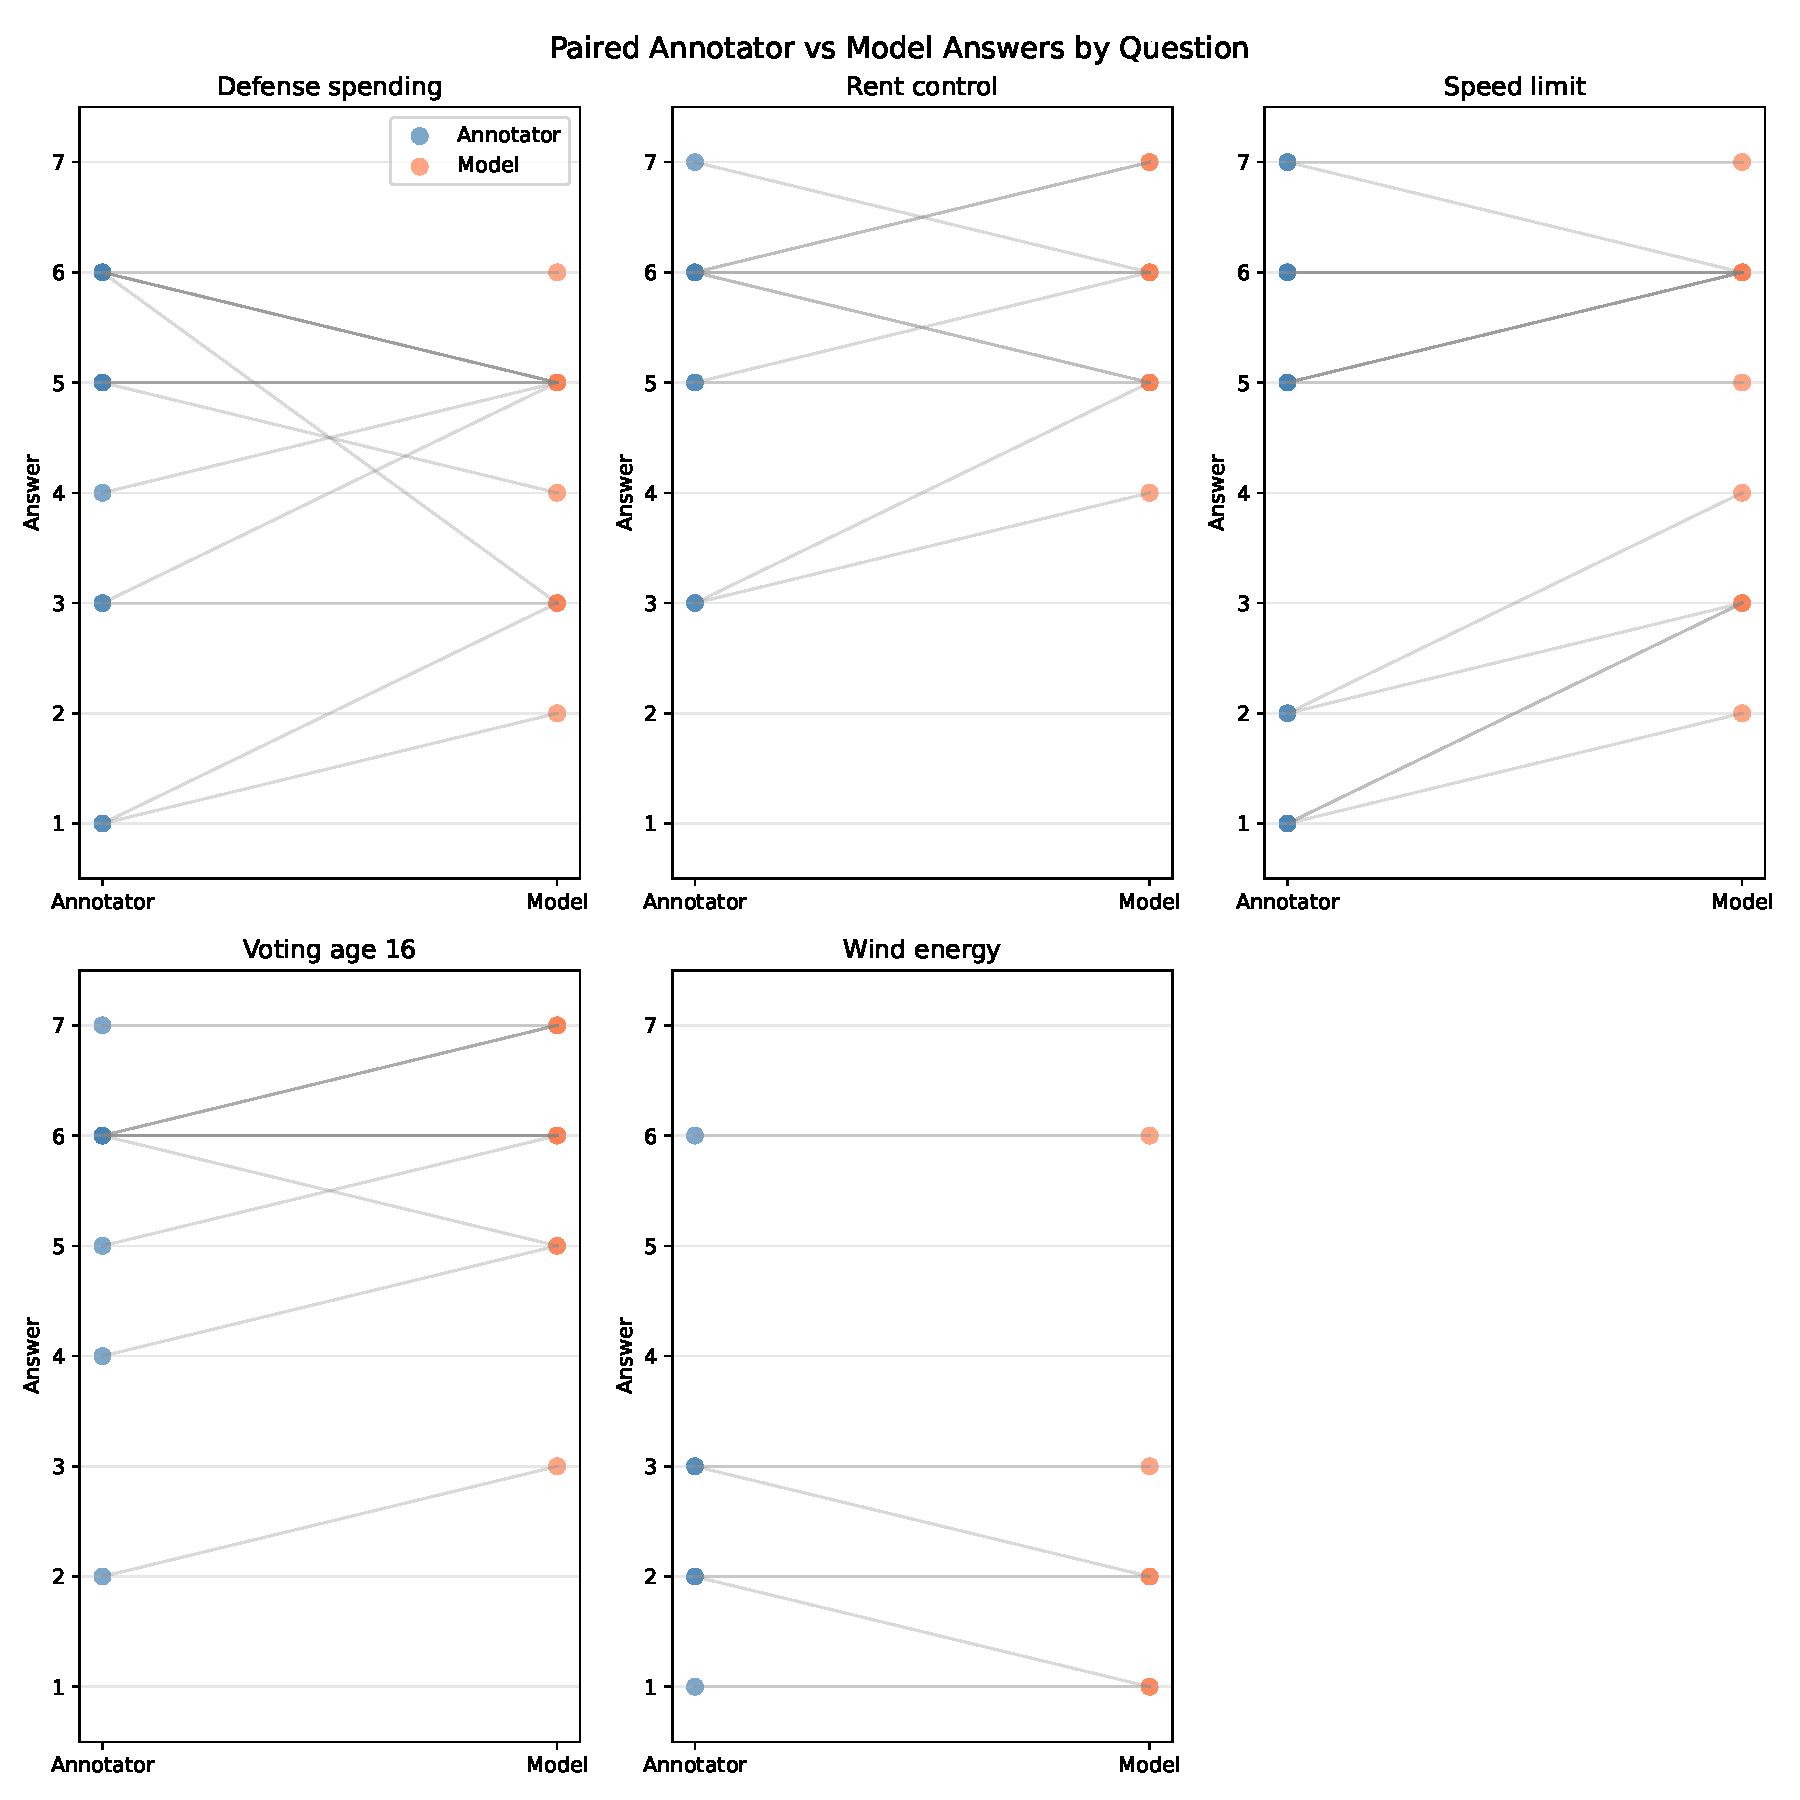
\includegraphics[width=\linewidth]{imgs/sanity_check_paired_plot.pdf}
\caption{Paired human and model ratings across questionnaire items. Lines connect corresponding observations; darker colours represent overlapping values.}
\label{fig:sanity_check}
\end{figure}


\section{Prompt Sensitivity - RQ1}


The Likelihood Ratio Test (LRT) was performed to compare the full model (Equation \ref{equ:full_model}) against the reduced model. The test yielded a highly significant result ($\chi^2(10) = 567.31, p < 0.0001$). This indicates that the model including the \texttt{prompt\_version} parameter provides a statistically significant better fit to the data than the model without it.

This finding confirms that the prompt phrasing has a significant influence on the agents' responses. Such sensitivity underscores the need for caution when designing experiments and interpreting results that rely on a single prompt version. This result supports our decision to employ a multi-prompt methodology, as it helps to mitigate potential biases introduced by any single phrasing.

It is important to note, however, that while this primary model showed a strong effect, two other models with different specifications were also analysed, and they yielded different results. This suggests the influence of prompt phrasing may be complex and potentially interact with other model assumptions, reinforcing the need for a robust, multi-prompt validation approach.


%\emptydoublepage

%% %%%%%%%%%%%%%%%%%%%%%%%%%%%%%%%%%%%%%%%%%%%%%%%%%%%%%%%%%%%%%%%%%%%%%%
%  ╭─────────╮                      ╔══╦╗ ╗ ╔═╦═╗ ╥ ┌─┐┌─┐┌─┐┬ ┬┌─┐┌┐ ┬
%  │ ,-= ━━━┑│                  |   ╠═╦╝╚╗╠╗║ ║ ╠═╣ ├─┤├─┤│  ├─┤├─ │└┐│
%  │ % iTec  │                  |   ╨ ╚═ ╚╝╚╝ ╨ ╨ ╨ ┴ ┴┴ ┴└─┘┴ ┴└─┘┴ └┘
%  │┃°. .°.  │ Chair Individual |          ┬ ┬┌┐ ┬┬┬  ┬┌─┐┬─┐┌─┐┬┌┬┐┬ ┬
%  │┖  °   ° │   and Technology |          │ ││└┐││└┐┌┘├─ ├┬┘└─┐│ │ └┬┘
%  ╰─────────╯                             └─┘┴ └┘┴ └┘ └─┘┴└─└─┘┴ ┴  ┴
% %%%%%%%%%%%%%%%%%%%%%%%%%%%%%%%%%%%%%%%%%%%%%%%%%%%%%%%%%%%%%%%%%%%%%%
%  This file is part of the Master's thesis LaTeX template used at the
%  Chair Individual and Technology (iTec) at RWTH Aachen University.
% %%%%%%%%%%%%%%%%%%%%%%%%%%%%%%%%%%%%%%%%%%%%%%%%%%%%%%%%%%%%%%%%%%%%%%


%% %%%%%%%%%%%%%%%%%%%%%%%%%%%%%%%%%%%%%%%%%%%%%%%%%%%%%%%%%%%%%%%%%%%%%
\chapter{Discussion}
\label{chap:discussion} 


%% %%%%%%%%%%%%%%%%%%%%%%%%%%%%%%%%%%%%%%%%%%%%%%%%%%%%%%
\section{Discussion of Results}
\label{sec:discussion-of-results}


%% %%%%%%%%%%%%%%%%%%%%%%%%%%%%%%%%%%%%%%%%%%%%%%%%%%%%%%
\section{Limitations}
\label{sec:limitations}


%% %%%%%%%%%%%%%%%%%%%%%%%%%%%%%%%%%%%%%%%%%%%%%%%%%%%%%%
\section{Future Work}
\label{sec:future-work}


%\emptydoublepage

%% %%%%%%%%%%%%%%%%%%%%%%%%%%%%%%%%%%%%%%%%%%%%%%%%%%%%%%%%%%%%%%%%%%%%%%
%  ╭─────────╮                      ╔══╦╗ ╗ ╔═╦═╗ ╥ ┌─┐┌─┐┌─┐┬ ┬┌─┐┌┐ ┬
%  │ ,-= ━━━┑│                  |   ╠═╦╝╚╗╠╗║ ║ ╠═╣ ├─┤├─┤│  ├─┤├─ │└┐│
%  │ % iTec  │                  |   ╨ ╚═ ╚╝╚╝ ╨ ╨ ╨ ┴ ┴┴ ┴└─┘┴ ┴└─┘┴ └┘
%  │┃°. .°.  │ Chair Individual |          ┬ ┬┌┐ ┬┬┬  ┬┌─┐┬─┐┌─┐┬┌┬┐┬ ┬
%  │┖  °   ° │   and Technology |          │ ││└┐││└┐┌┘├─ ├┬┘└─┐│ │ └┬┘
%  ╰─────────╯                             └─┘┴ └┘┴ └┘ └─┘┴└─└─┘┴ ┴  ┴
% %%%%%%%%%%%%%%%%%%%%%%%%%%%%%%%%%%%%%%%%%%%%%%%%%%%%%%%%%%%%%%%%%%%%%%
%  This file is part of the Master's thesis LaTeX template used at the
%  Chair Individual and Technology (iTec) at RWTH Aachen University.
% %%%%%%%%%%%%%%%%%%%%%%%%%%%%%%%%%%%%%%%%%%%%%%%%%%%%%%%%%%%%%%%%%%%%%%


%% %%%%%%%%%%%%%%%%%%%%%%%%%%%%%%%%%%%%%%%%%%%%%%%%%%%%%%%%%%%%%%%%%%%%%
\chapter{Conclusion}
\label{chap:conclusion} 


shall answer the main question "So what?"

why did we do what we did and what did we learn from it.

%\emptydoublepage


%% %%%%%%%%%%%%%%%%%%%%%%%%%%%%%%%%%%%%%%% 
 \begin{appendix}
 

\chapter{Types of harm}
\label{abc}
\begin{table}[h!]
    \centering
    \renewcommand{\arraystretch}{1.3}
    \begin{tabular}{|p{4cm}|p{10cm}|}
        \hline
        \multicolumn{2}{|c|}{\textbf{Representational Harms}} \\
        \hline
        \textbf{Type of Harm} & \textbf{Definition} \\
        \hline
        \textbf{Derogatory language} & Pejorative slurs, insults, or phrases that target and denigrate a social group.\\
        \hline
        \textbf{Disparate system performance} & Degraded understanding, diversity, or richness in language processing or generation between social groups.
         \\
        \hline
        \textbf{Erasure} & Omission or invisibility of the language and experiences of a social group.
        \\
        \hline
        \textbf{Exclusionary norms} & Reinforced normativity of the dominant social group and implicit exclusion or devaluation of other groups.  \\
        \hline
        \textbf{Misrepresentation} & An incomplete or non-representative distribution of the sample population generalized to a social group. \\
        \hline
        \textbf{Stereotyping} & Negative, generally immutable abstractions about a labeled social group. \\
        \hline
        \textbf{Toxicity} & Offensive language that attacks, threatens, or incites hate or violence against a social group. \\
        \hline
        \multicolumn{2}{|c|}{\textbf{Allocational Harms}} \\
        \hline
        \textbf{Type of Harm} & \textbf{Definition} \\
        \hline
        \textbf{Direct discrimination} & Disparate treatment due explicitly to membership of a social group. \\
        \hline
        \textbf{Indirect discrimination} & Disparate treatment despite formally neutral consideration towards social groups, due to proxies or other implicit factors. \\
        \hline
    \end{tabular}
    \caption{Types of Representational and Allocational Harms by \citet[p.1103]{gallegos_bias_2024}}
    \label{tab:harms}
\end{table}

% \emptydoublepage
% \include{appendix_02}
% \emptydoublepage
 \end{appendix}

%% %%%%%%%%%%%%%%%%%%%%%%%%%%%%%%%%%%%%%%%%%%%%%%%%%%%%%%
\backmatter

%% %%%%%%%%%%%%%%%%%%%%%%%%%%%%%%%%%%%%%%%
%%  Bibliography
\clearpage
\phantomsection
\addcontentsline{toc}{chapter}{\protect\numberline{}Bibliography}
 \bibliographystyle{plainnat}
%\bibliographystyle{IEEEtranN}
%\bibliographystyle{apa}
\bibliography{thesis}
\emptydoublepage

%% %%%%%%%%%%%%%%%%%%%%%%%%%%%%%%%%%%%%%%%
%%  Index
%\markboth{Index}{Index}
%\thispagestyle{plain}
%\phantomsection
%\addcontentsline{toc}{chapter}{\protect\numberline{}Index}
%\printindex

%% %%%%%%%%%%%%%%%%%%%%%%%%%%%%%%%%%%%%%%%
%date of typesetting
\newpage
\thispagestyle{empty}
\vspace*{\fill}
\hspace*{\fill}{\tiny Typeset \today}

%% %%%%%%%%%%%%%%%%%%%%%%%%%%%%%%%%%%%%%%%%%%%%%%%%%%%%%%%%%%%%%%%%%%%%%
\end{document}
%% %%%%%%%%%%%%%%%%%%%%%%%%%%%%%%%%%%%%%%%%%%%%%%%%%%%%%%%%%%%%%%%%%%%%%%%%%%%
